% !TeX root = RJwrapper.tex
\title{\pkg{IndexNumber}: An R Package for Measuring the Evolution of Magnitudes}
\author{by Alejandro Saavedra-Nieves and Paula Saavedra-Nieves}

\maketitle

\abstract{
Index numbers are descriptive statistical measures useful in economic settings for comparing simple and complex magnitudes registered, usually in two time periods. Although this theory has a large history, it still plays an important role in modern today's societies where big amounts of economic data are available and need to be analyzed. After a detailed revision on classical index numbers in literature, this paper is focused on the description of the R package \CRANpkg{IndexNumber} with strong capabilities for calculating them. Two of the four real data sets contained in this library are used for illustrating the determination of the index numbers in this work. Graphical tools are also implemented in order to show the time evolution of considered magnitudes simplifying the interpretation of the results.
}
\vspace*{-0.25 cm}
\section{Introduction}


The problem of reducing a large amount of available microeconomic data is common in dynamic and modern economies. Individuals of today's societies consume services of hundred of commodities over a year, and most producers use and produce hundreds of individual products and services. This overwhelming abundance of data is usually summarized through index numbers theory. \emph{Index numbers} are descriptive statistical measures useful in order to compare or measure changes in simple and complex magnitudes over time. The goal is usually to determine possible increases or decreases and, more generally, trend changes. The situations to be compared are in no way restricted; they may be two time periods (hours, days, months, or years); two places (two cities or countries); or two groups of people (economically active and inactive population). For simplicity in the exposition, we  refer to temporal index numbers in this paper. The rest of the situations mentioned could be considered modifying the notation slightly.  

Although index numbers are considered a classical statistical tool, the problem of how to construct them is as much one of economic theory as of statistical technique, see \cite{frisch1936annual}. This can be checked by analyzing their considerable history.  Initial works involving index numbers date back to the early 18th century.  During the creation of a college in 1440–1460, it was stipulated that any member had to leave it if his richness exceeded five pounds per year. The Anglican Bishop Fleetwood desired to know if, according to the price evolution, this promise could be kept three centuries later. Then, he studied the evolution of prices corresponding to four products (wheat, meat, drink, and clothing) from 1440 to 1700.  He concluded that five pounds in 1440–1460 had the same value as 30 pounds in 1700. More details can be found in \cite{fleetwood1707chronicon}. \cite{de1754reflexions} studied the diminution of the money value analyzing the incomes of kings Louis XII and Louis XV. In order to know which of them had the largest disposable income, he considered the prices of several goods of different nature as such as a chicken, a rabbit, a pigeon, or the day’s work value.  From the discovery of the Americas, the astronomy professor of Padoue analyzed the evolution of prices in 1764. He considered the prices of three commodities (grains, wine, and cooking oil), and he studied their variation from 1500 to 1750.  \cite{evelyn1798account} can be seen as a precursor of index numbers establishing a price index number from 1050 to 1800. In this work, notions as the year of reference and relative prices were introduced.  According to \cite{kendall}, the real father of index numbers is Joseph Lowe. Many problems dealing with their construction were presented in \cite{lowe1822present}. In fact,  Lowe's measurement would be known as the Laspeyres index later. In the second half of the 19th century, statisticians developed many advances in this setting.  \cite{jevons1863serious} recommended considering the geometrical mean in order to construct an index number. Between 1864 and 1880, \cite{laspeyres1864hamburger, laspeyres1871ix}, \cite{drobisch1871ueber}, and \cite{paasche1874ueber} worked on the evolution of prices for material goods from the approach of  weighted index numbers.  \cite{palgrave1886currency} proposed to weigh the relative prices by the total amount of the considered good. \cite{fisher1922making} defined a new index number calculated as the geometric mean of the Laspeyres and the Paasche index numbers. In the same period, Marshall and Edgeworth proposed to calculate weighted means.  For an in-depth review on this topic, see \cite{kendall1969studies}, \cite{allen1982index} or more recently, \cite{manual2004consumer}, or \cite{dodge2008concise}.  

Nowadays, economists continue to use index numbers to make comparisons over time despite their long background. In fact, the main applications of index numbers are either economic, or they occur in related fields as demography or technology. In such settings, the magnitudes to be compared through index numbers usually come in pairs, one of price and the other a matching one of quantity. This pair may be designed to account for the variation in an aggregate value, as when movements in the aggregated expenditure of consumers are analyzed into the two components of changes in prices and in  real consumption. Some more recent contributions in index numbers theory are exposed next. \cite{barnett1980economic} focused on economic monetary aggregates from this approach. Changes in food prices were analyzed in \cite{lamm1980index}. Index numbers in chain, or more commonly chain indices, are considered in \cite{forsyth1981theory}. \cite{boyle1988economic} analyzed the volume of Irish agricultural output from 1960 to 1982. Scanner data on coffee sales are studied in \cite{de1997estimation}.  \cite{hill1999comparing} shows how a comparison of price levels across a group of countries can be made by chaining Fisher index numbers across a spanning tree. Inequality and poverty in several regions of Thailand are studied through the construction of urban and rural cost of living and welfare indices in \cite{kakwani2002economic}. \cite{dumagan2002comparing} showed that the  Fisher index could be numerically approximated by other superlative index numbers. In \cite{reinsdorf2002additive}, additive decompositions of the Fisher index are derived in order to know how much each item contributes to its overall change. From data from United States, Canada, France, Germany, Italy, Japan, and the United Kingdom, drug price and quantity index numbers are considered in \cite{danzon2000cross}. \cite{ang2004generalized} used a generalized version of the Fisher index to analyze CO$_2$ emission. In \cite{boyd2004note}, the structural change in energy intensity is studied. Exploring the duality between a return to dollar definition of profit and the generalized distance function, the relationship between the Laspeyres, Paasche and Fisher productivity index numbers is established in \cite{zofio2006return}. \cite{hill2006does} showed an illustration on index numbers also using scanner data. An application to major crops in Manitoba is presented in \cite{coyle2007aggregation}. According to \cite{diewert2007measurement}, Paasche, Laspeyres, or Fisher index number formula is useful in order to manage the total factor productivity growth. The importance of the hedonic imputation method in price index numbers is analyzed in \cite{hill2008hedonic} from a data set containing house prices for three regions in Sydney over a three years period. The impact of time aggregation on price change estimates for several supermarket item categories is considered in \cite{ivancic2011scanner}. \cite{bialek2012proposition} proposed a general price index formula with the Fisher, Laspeyres, and Paasche indices as its particular cases. \cite{bialek2014simulation} presented an original price index, and its performance is analyzed through a simulation study where it is compared to several classical price index numbers.  A generalized version of the Fisher index is considered in \cite{su2014attribution} in order to analyze changes in the carbon emissions embodied in China's exports. \cite{o2018measures} analyzed the productivity change defined as measures of output quantity change divided by measures of input quantity change.  \cite{zhen2019scanner} constructed panel price index numbers using retail scanner data in order to compare consumption costs across space and time.

This paper is focused on the description of the R package \CRANpkg{IndexNumber} \citep{SN}, available from the \emph{Comprehensive R Archive
Network} at \url{https://CRAN.R-project.org/package=IndexNumber}, and its capabilities for calculating classical index numbers. It is organized as follows. Index numbers are formally defined in Section \ref{sec1}. Section \ref{si} introduces simple index numbers. Concretely, simple index numbers in series and in chain are distinguished. In Section \ref{cin}, non-weighted and weighted complex index numbers are presented. Details on the usage of \pkg{IndexNumber} package are considered from Section \ref{indexnumberinpractice}. The four real data sets contained in the library are also described briefly. Note that two of them are used in this paper in order to illustrate the calculation of index numbers. They are available on the website of the \emph{Spanish Statistical Office (INE)}, \url{http://www.ine.es}.



\vspace{-0.3 cm}
\section{Preliminaries on index numbers}\label{sec1}

\emph{Index numbers} are statistical measures that are useful to compare single and multiple magnitudes for the same interval of time. In both cases, this comparison is made with respect to an element of the mentioned series that is called base period or reference. 
Some examples of simple magnitudes are prices of a good, sold amounts of a product,  or other general individual values.  However, most of the time,  comparing these simple quantities has not practical interest. If the goal is to analyze some real phenomena where many variables are involved, complex indices must be considered. Using these ideas,  index numbers are usually classified into the following two groups:\vspace{-0.15 cm}

\begin{itemize}
\item An index number is said to be simple if it corresponds to the ratio of two values of the same variable, measured in two different instants. Therefore, a \emph{simple index number} provides the variation that the single magnitude has suffered between two different time periods. 

For instance, a simple index number of the price will give the relative variation of the price between the current period and the period taken as reference. 

\item Most of the time,  comparing prices, amounts, or  values of a single product individually is not of interest in practice. If the goal is to analyze some real situations where different variables have influence, a \emph{complex number index} has to be considered. It globally summarizes the information of the different magnitudes involved in the problem. 

For instance, the evolution cost of life in a country is a common case where it is necessary to select a set of goods or variables that give information about it. The relative importance of each of the goods considered must be measured and taken into account.
\end{itemize}

% They are able to summarize the %information of the different indexes related to the variables taken into account. A very well-knwon example is the %analysis of the evolution cost of the life in a country. Here, it is necessary to select a set of goods or variables %giving information about the cost. The relative importance of each of the goods considered must be taken into account. %The Consumer Price Index (CPI) in Spain for the last four months of year 2019 is shown in Table \ref{IPCspain}. The %items in the consumption basket used in its calculation are grouped in subclasses, these in classes, then in subgroups %and, finally, the subgroups are added in groups. This classification is fully adapted to the international %classification of consumption COICOP (Classification of Individual Consumption according to Purpose), prepared by the %Statistical Division of the United Nations. In this way, comparisons between different countries can be easily %performed. Table \ref{IPCspain} contains some of the groups considered for determining the CPI value. Concretely, $X_1$ %refers to  foodstuff and non-alcoholic drinks; $X_2$, alcoholic drinks and tobacco; $X_3$, clothing and footwear; $X_4$, %housing, water, electricity, gas and other fuels; $X_5$, furniture, home objects and maintenance home items; $X_6$, %health service. The goal is to obtain a simple index number that summarizes the biggest amount of information. This %dataset is available from the webpage of the Spanish Statistics National Institute (INE), \url{www.ine.es}.


%\begin{table}[h!]\centering
%	\begin{tabular}{|l||cccccccc|}\hline
%		Stages & CPI & $X_1$& $X_2$ &$X_3$& $X_4$& $X_5$& $X_6$& ...\\\hline
%		2019M12	&105,228	&105,065	&103,991	&112,023&	102,826	&100,781&	102,073&	...\\
%		2019M11&	105,304&	105,24&	104,332&	114,421&	104,011&	100,912&	102,047&	...\\
%		2019M10& 	105,126	&105,276	&104,378&	109,108&	104,472&	100,72&	101,983&	...\\
%		2019M09	&104,116&	103,732&	104,341&	98,14&	103,378&	100,224&	101,887&	...\\
%		...	&...	&...	&...	&	...	&...	&...	&	...	&	...	\\
%		\hline
%	\end{tabular}\caption{CPI value in Spain and some of the groups considered in the Classification of Individual Consumption according to Purpose.}\label{IPCspain}\end{table}




%Two important features are must be taken into account to make comparisons in this setting. First, it is necessary to establish the initial situation. All comparisons will be refered to this value. Therefore, it must be selected carefully according to the goals established. Secondly, the magnitudes to be compared can be simple or complex. An example of complex magnitude is to compare the industrial production of a specific country in two different times. Note that production units, litres or kilograms should be considered in order to study the total industrial production. Therefore, a complex magnitude can be seen as a set of several heterogeneous simple magnitudes.

A wider overview of both classes of index numbers is included in the  next sections. In particular, we distinguish the different subclasses belonging to each of them and their possible relationships.


%METER AQUI PROPIEDADES DE LOS NUMEROS INDICES: EXISTENCIA, IGUALDAD, INVERSION, CIRCULAR, CICLICA, PROPORCIONALIDAd, PAGE 14

\subsection{Simple index numbers}\label{si}

A \emph{simple index number} is a statistical indicator of the percentage of variation of a single magnitude in two different instants. Simple index numbers are usually classified according to the element that we take as reference.  In particular, we distinguish two types of simple index numbers. First, we describe simple index numbers in series, when the first value of the series is taken as the reference value, and simple index numbers in chain (or chain indices), when the reference is the immediately previous value in the serie. 

In what follows, we assume that $X=\{x_0,x_1,\dots,x_T\}$ denotes the observations of the magnitude $X$ for the $T+1$ time instants considered. Besides, $x_0$ is usually taken as the base period. Most common simple index numbers are individually referred to variables in real-world situations as the followings:
\begin{itemize}
	\item  the \emph{price of a good}, denoted by $p$;
	\item  the \emph{amount  of produced or sold product}, denoted by $q$; or
	\item the \emph{value of a good}, denoted by $v$. This value is usually obtained as the product of the price and the amount variables.
\end{itemize}

In this section, we illustrate the usage of simple index numbers on a real example. Table \ref{tab0} shows the number (thousands) of economically active women and men in Spain from the first trimester of 2002 (taken as a reference value). Remark that four trimesters of each year are denoted by T1, T2, T3 and T4, respectively. 

\vspace*{-0.1 cm}\begin{table}[h!]\centering\resizebox{\textwidth}{!}{
		\begin{tabular}{|l||ccccccc|}\hline
			Stages &       2002 (T1)&   2002 (T2) &  2002 (T3) &   2002 (T4)&  2003 (T1)&2003 (T2)&...\\\hline
			Total of women  &     7442.70& 7580.80& 7670.20 &7751.50& 7868.70& 7977.80&...\\ 
			Total  of men &     11192.30 &11289.40 &11445.10& 11472.80& 11552.50& 11661.40&...\\\hline
	\end{tabular}}\caption{Number (thousands) of  economically active women and men in Spain from first trimester of 2002.}\label{tab0}\end{table}

This dataset, included in \pkg{IndexNumber} package, can be obtained from the Economically Active Population Survey (EPA) elaborated by the Spanish Statistics National Institute (INE). 


\subsubsection{Simple index numbers in series}\label{siserie}

Let $x_0$ and $x_t$ be the values of the variable $X$ where $x_0$ corresponds to the base period and  $t\in \{0,1,\dots,T\}$,  respectively.  Thus, the value of the simple index number in series for $X$ in $t$ is defined as follows:
\begin{equation}\label{niinserie}
I_0^t(X)=\frac{x_t}{x_0}\cdot 100.
\end{equation}
For each  $t\in \{0,1,\dots,T\}$, this measure has a natural interpretation. Fixed a certain variable of interest $X$, the index number in series in $t$ shows the percentage of variation of the magnitude in this instant of time with respect to the reference value (in this case, the initial one). 

Using this type of index number, some usual magnitudes can be formally defined as it is indicated next: 
\begin{itemize}
	\item When  prices are considered, the \emph{relative price} of a product $i$, also called simple price index, can be determined as\vspace*{-0.05 cm} $$p_0^t=\frac{p_{it}}{p_{i0}},\vspace*{-0.05 cm}$$where $p_{it}$ denotes the price at instant $t$ and $p_{i0}$, the price in the base period. 
	\item The \emph{relative amount} of a product $i$ can be written as \vspace*{-0.05 cm} $$q_0^t=\frac{q_{it}}{q_{i0}},\vspace*{-0.05 cm}$$ where $q_{it}$ denotes the produced or sold amount at instant $t$ and $q_{i0}$, the amount for the base period. 
	\item Finally, the \emph{relative value} of a product $i$ has the next expression:\vspace*{-0.05 cm}$$v_0^t=\frac{v_t}{v_0}=\frac{p_{it}q_{it}}{p_{i0}q_{i0}}\cdot 100= p_0^t\cdot q_0^t\cdot 100,\vspace*{-0.05 cm}$$ where $v_{t}$ denotes the value of the good at instant $t$ and $v_{0}$, the value of the base period. 
\end{itemize}




Below, we illustrate the usage of simple index numbers on the two series included in Table \ref{tab0}. Thus, the simple index numbers in series for the economically active women and men in Spain from the first trimester of 2002 is given in Table \ref{tab1}. 

\begin{table}[h!]\centering\resizebox{0.99\textwidth}{!}{
\begin{tabular}{|l||ccccccc|}\hline
Stages &       2002 (T1)&   2002 (T2) &  2002 (T3) &   2002 (T4)&  2003 (T1)&2003 (T2)&...\\\hline
Index number for women & 100.00 & 101.86&  103.06&  104.15&  105.73&  107.19& ...\\
Index number for men &  100.00&   100.87 &  102.26&   102.51&   103.22&   104.19&...\\\hline
	\end{tabular}}\caption{Simple index numbers in series for number (thousands) of  economically active women and men in Spain from the first trimester of 2002.}\label{tab1}\end{table}



 


Comparing the evolution of the index numbers in series for the population of women and men shown in Table \ref{tab1}  has an interest, for instance, to analyze the effect of variable sex in the Spanish labor market. Note that the number of economically active women and men in the second trimester of 2003 is 7.2\% and 4.2\% larger than in the reference time, respectively. Therefore, women increasing is slightly larger than men.



\subsubsection{Simple index numbers in chain}\label{sichain}

Below, we introduce another approach of simple index numbers. Contrary to our previous assumptions,  this new setting arises when the reference value is not the initial one; rather we take the value immediately preceding. Let $x_{t}$ and $x_{t-1}$ be two values of a variable $X$ observed in two consecutive instants $t$ and $t-1$, being $t\in \{1,2,\dots,T\}$. Thus, the value of the \emph{index number in chain} or \emph{chain index} (cf. \citealp{forsyth1981theory}) that corresponds to an instant $t$, with $t\in \{1,2,\dots,T\}$, is defined as follows:
\begin{equation}\label{niinchain}
IC^t(X)=\frac{x_t}{x_{t-1}}\cdot 100.
\end{equation}
Again, this index number can be naturally interpreted. It is worth  mentioning that these measures the variation of the characteristic under study with respect to the previous value in a fixed instant $t$. For instance, these index numbers reflect the percentage variation that the variable experiments between two consecutive values in time series settings.

To illustrate this definition, we take again the example considered in the previous section. For this subset of values, we obtain again the evolution of the amount of economically active people (per sex) in Spain under this new approach.

\vspace*{-0.1 cm}\begin{table}[h!]\centering\resizebox{0.99\textwidth}{!}{
		\begin{tabular}{|l||ccccccc|}\hline
			Stages &       2002 (T1)&   2002 (T2) &  2002 (T3) &   2002 (T4)&  2003 (T1)&2003 (T2)&...\\\hline
Index number for women& 100.00  &101.86 & 101.18  &101.06 & 101.51  &101.39& ...\\
			Index number for men&   100.00 &  100.87 &  101.38 &  100.24&   100.70&   100.94&...\\			
			\hline
	\end{tabular}}
	\caption{Simple index numbers in chain for number (thousands) of economically active women and men in Spain from the first trimester of 2002.}\label{tab4}\end{table}

 
Table \ref{tab4} shows the evolution in time of the number (thousands) of economically active women and men in Spain from the  trimester of 2002 (see Table \ref{tab0}). According to the obtained results, we emphasize as relevant that the number of economically active women and men in the second trimester of 2003 increases 1.4\% and 0.9\%, respectively, with respect to the previous trimester.  



\vspace*{0.2 cm}\noindent\textbf{Relationship between simple index numbers in series and in chain}

\noindent This section briefly introduces some comments on the relations between simple index numbers in series and in chain. In this way, one can be obtained from  another (and vice versa) without having to use the exact values of the magnitude under study.  

Take $x_t$ the value of the variable $X$  in  instant $t$, with $t\in \{1,2,\dots,T\}$. Thus, a simple index in chain can be obtained from a simple index in series due to the relation\vspace*{-0.05 cm}
\[IC^t(X)=\frac{x_t}{x_{t-1}}\cdot 100= \frac{\frac{x_t}{x_0}}{\frac{x_{t-1}}{x_0}}\cdot 100=\frac{I_0^t(X)}{I_0^{t-1}(X)}\cdot 100.\vspace*{-0.05 cm}\]
For example, from simple index numbers in series for women shown in Table \ref{tab1}, it is possible to obtain the corresponding simple index number in chain for women also for the first trimester of 2003 (contained in Table \ref{tab4}). That is,\vspace*{-0.05 cm}
$$IC^{2003(T1)}(X)=\frac{7868.70}{7751.50}\cdot 100=\frac{105.72}{104.15}\cdot 100=101.51.\vspace*{-0.05 cm}$$

Besides, simple indices in series can be equivalently obtained for each $t\in \{1,\dots,T\}$ from indices in chain:\vspace*{-0.05 cm}
$$I_0^t(X)=\frac{x_t}{x_{0}}\cdot 100=\frac{x_t}{x_{t-1}}\frac{x_{t-1}}{x_{t-2}}\cdots   \frac{x_2}{x_{1}}\frac{x_1}{x_{0}} \cdot 100=\frac{IC^t(X)}{100}\cdot\frac{IC^{t-1}(X)}{100}\cdot \cdots \cdot \frac{IC^{2}(X)}{100}\cdot \frac{IC^{1}(X)}{100}\cdot 100. \vspace*{-0.05 cm}$$
For instance, if we consider the simple index numbers in chain shown in Table \ref{tab4}, it is possible to obtain the simple index number in series for the first trimester of 2003 contained in Table \ref{tab1}. That is, we check that\vspace*{-0.05 cm}
$$I_0^{2003(T1)}(X)=   \frac{100.70}{100} \cdot \frac{100.24}{100}    \cdot \frac{101.38}{100}    \cdot \frac{100.87}{100} \cdot 100.\vspace*{-0.05 cm} $$



\vspace*{0.1 cm}\noindent\textbf{Variation Rate}

\noindent In this section, we formally introduce another measure of the evolution of a magnitude. Furthermore, we relate it to the simple index numbers previously defined.

The \emph{variation rate} of the  observations in the instants $t$ and $t-1$, with $t\in \{1,\dots,T\}$, is denoted by $\mbox{Rate}^t(X)$ for each $t\in\{1,\dots,T\}$. It can be calculated from the simple index in chain as follows:
$$\mbox{Rate}^{t}(X)=\frac{x_{t}-x_{t-1}}{x_{t-1}}\cdot100=IC^t(X)\cdot 100.$$This definition can be extended to any pair of instants in $\{0,1,2,\dots,T\}$. Take $t_1, t_2\in \{0,1,2,\dots,T\}$ such that $t_1<t_2$. Let $x_{t_1}$ be the value of a variable measure in instant $t_1$ and let $x_{t_2}$ be the value of a variable measure in a later instant $t_2$. Formally, the \emph{variation rate} of $X$ in $t_2$ with respect to $t_1$ is\vspace*{-0.05 cm} $$\mbox{Rate}_{t_1}^{t_2}(X)=\frac{x_{t_2}-x_{t_1}}{x_{t_1}}\cdot 100.\vspace*{-0.05 cm}$$
Note that\vspace*{-0.05 cm}$$\mbox{Rate}_{t_1}^{t_2}(X)=\frac{x_{t_2}-x_{t_1}}{x_{t_1}}\cdot 100=\left(\frac{x_{t_2}}{x_{t_1}}-1\right)\cdot 100 = I_{t_1}^{t_2}(X)-100,\vspace*{-0.05 cm}$$
where $I_{t_1}^{t_2}(X)=\frac{x_{t_2}}{x_{t_1}}\cdot 100$, also satisfying\vspace*{-0.05 cm}
\[I_{t_1}^{t_2}(X)=IC^{t_2}(X)\cdot IC^{t_2-1}(X)\cdot \mbox{ }\dots\mbox{ } \cdot IC^{t_1+1}(X).\vspace*{-0.05 cm}\]In particular, if the consecutive observations correspond to two different years, months, or trimesters the variation rate is called interanual variation rate, monthly variation rate, and quarterly variation rate, respectively. From the data shown in Table \ref{tab1}, the quarterly variation rates have been calculated in Table \ref{tabrateh}.
\begin{table}[h!]\centering\resizebox{0.8\textwidth}{!}{
		\begin{tabular}{|l||cccccc|}\hline
			Stages &         2002 (T2) &  2002 (T3) &   2002 (T4)&  2003 (T1)&2003 (T2)&...\\\hline
			Rate for women  &1.86& 1.18& 1.06& 1.51& 1.39&...\\
			Rate for men   & 0.87& 1.38& 0.24 &0.70& 0.94&...\\			
			 \hline
	\end{tabular}}\caption{Quarterly variation rate for number (thousands) of economically active women and men in Spain.}\label{tabrateh}\end{table}



\vspace*{0.1 cm}\noindent\textbf{Average Variation Rate}

\noindent Finally, we introduce a third method to measure the evolution of a given magnitude $X$ between the instants $t$ and $t+k$, with $t \in \{0,\dots,T-k\}$ and $k>0$.  If $x_{t+k}$ denotes the observation at instant $t+k$ and $x_t$ the corresponding to instant $t$, the \emph{average variation rate} of the variable $X$ between instants $t$ and $t+k$ is defined as the constant rate $T_k$ that allows obtaining the observation $x_{t+k}$ at time $t+k$ from observation $x_t$ at time $t$. 

Then, it is possible to write:
\begin{equation*}
\begin{split}
x_{t+1}&=x_t+\frac{T_k}{100}\cdot x_t=\left(\frac{100+T_k}{100}\right)\cdot x_t\\
x_{t+2}&=x_{t+1}+\frac{T_k}{100}\cdot x_{t+1}=\left(\frac{100+T_k}{100}\right)^2\cdot x_t\\
\end{split}
\end{equation*}
\begin{equation*}
\begin{split}
x_{t+3}&=x_{t+2}+\frac{T_k}{100}\cdot x_{t+2}=\left(\frac{100+T_k}{100}\right)^2\cdot x_t\\
& \vdots\\
x_{t+k}&=x_{t+k-1}+\frac{T_k}{100}\cdot x_{t+k-1}=\left(\frac{100+T_k}{100}\right)^k\cdot x_t
\end{split}
\end{equation*}\vspace*{-0.05 cm}
Therefore, $x_{t+k}=\left(\frac{100+T_k}{100}\right)^k \cdot x_t$ and, as consequence, $\frac{x_{t+k}}{x_t}=\left(\frac{100+T_k}{100}\right)^k.$ Then,\vspace*{-0.05 cm}
$$T_k=100\cdot\left(\frac{x_{t+k}}{x_t} \right)^{1/k}.\vspace*{-0.05 cm}$$
From data shown in Table \ref{tab1},  we have calculated the quarterly average variation rate in $2002$ for women and men as\vspace*{-0.05 cm}
 $$\left(\sqrt[3]{\frac{7751.50}{7442.70}}-1\right)\cdot 100 = 1.36 \mbox{ and }\left(\sqrt[3]{\frac{11472.80}{11192.30}}-1\right)\cdot 100=0.83\mbox{, respectively.}\vspace*{-0.05 cm}$$According to the results obtained, the average variation rate for women is considerably bigger than the corresponding for men in this period.
 

\subsection{Complex index numbers}\label{cin}

Most of the time, comparing variables marginally does not provide real information. There are many phenomena in the real world that involve several variables. Of course, simple index numbers described in the previous section could be naturally applied for each of these variables separately. However, comparing these magnitudes can be not realistic and, for this reason, \emph{complex index numbers} have to be introduced. A complex index number summarizes the information of the different marginal index numbers related to the set of variables of interest. 

One of the most relevant examples that illustrates the use of complex index numbers is briefly  described next. The evolution  of living cost in a country is a common case where it is necessary to select a set of goods or variables that give information about it. The relative importance of each of the goods considered may be taken into account. This is the case of the \emph{Consumer Price Index} (CPI) in Spain. The sets of good considered for calculating it follows the \emph{International Classification of Consumption according to Purpose} (COICOP) prepared by the Statistical Division of the United Nations. This classification is also used by other countries. In this way, comparisons between different geographical areas make sense. 

When all variables are not of equal relevance, it is possible to add complementary information for weighting each magnitude corresponding to its degree of importance. Depending on the use of this additional information,  two classes of complex index numbers are distinguished in literature:

\begin{itemize}
	\item In several practical cases, the relative weight of each involved variable has no interest. Fixed a magnitude, the class of required index numbers to be used in this setting are named \emph{non-weighted complex index numbers}. 
\item The use of \emph{weighted index numbers} allow greater importance to be attached to some items. For instance, real information other than simply the change in price over time can be used. Factors as quantity sold or quantity consumed for each item can also be  considered.
\end{itemize}

In what follows, we assume that $X=(X_1,\dots,X_n)$ denotes the collection of $n$ magnitudes registered for $n$ different products. For each $j=1,\dots,n$, $X_j=\{x_{j0},x_{j1},\dots,x_{jT}\}$ denotes the observations of the magnitude $X_j$ for the  $T+1$ instants of time considered. Analogously to the simple case, we refer $x_{j0}$ as the base period.

In practice, the available information can be summarized in a table such as Table \ref{tab111}. 

	\begin{table}[h!]\centering\resizebox{0.45\textwidth}{!}{
	\begin{tabular}{|l||cccc|}\hline
	\backslashbox{Time}{Products} &     $1$&   $2$ &  ... &   $n$ \\\hline
	$0$  &     $x_{10}$&  $x_{20}$&  ...&  $x_{n0}$\\
	$1$  &     $x_{11}$&  $x_{21}$&  ...&  $x_{n1}$\\
	$\vdots$  &    $\vdots$&  $\vdots$& $\vdots$&  $\vdots$\\
	$T$  &     $x_{1T}$&  $x_{2T}$&  ...&  $x_{nT}$\\ \hline
	\end{tabular}}\caption{Evolution of a set of magnitudes $X$ from time $0$ to $T$.}\label{tab111}\end{table}

The most common complex indices jointly involve (some of) the variables in real-world situations that we enumerate below:
\begin{itemize}
	\item  the \emph{price of a collection of $n$ goods}, denoted by $p=(p_1,\dots,p_n)$, where $p_j=\{p_{j0},p_{j1},\dots,p_{jT}\}$ denotes the prices for $T+1$ instants and for each product $j=1,\dots,n$;
	\item  the \emph{amount  of produced or sold products}, denoted by $q$, where $q_j=\{q_{j0},q_{j1},\dots,q_{jT}\}$ denotes the amounts of product for $T+1$ instants and for each product $j=1,\dots,n$; or
%	\item the \emph{value of goods}, denoted by $v$. The value is usually obtained as the product of the price and the amount of units of each product.
	\item the \emph{value of $n$ goods} is given by $v=(v_1,\dots,v_n)$. In this case,  $v_j=\{v_{j0},v_{j1},\dots,v_{jT}\}$ denotes the values of product $j$, with $j\in \{1,\dots,n\}$ for $T+1$ instants.
\end{itemize}

To illustrate the usage of complex index numbers, we take the example described in Table \ref{tab1110}. It shows the unitary value (euros) of prices of combustibles and other energy resources for the main home in Spain from 2005 to 2015. In this case, the data source is again the Spanish Statistics National Institute (INE).

\small{
	\begin{table}[h!]\centering\resizebox{0.94\textwidth}{!}{
		\begin{tabular}{|l||ccccc|}\hline
			&Electricity &Natural municipal& Liquified &Liquified &Solid\\
			&(Kwh)       & gas ($m^3$)& gas (kilo) &combustibles (litre) &combustibles (kilo)\\
			\hline
			2006 &0.14 &0.70 &1.00 &0.69& 0.12\\ 
			2007 &0.14& 0.78 &0.97 &0.66 &0.10\\ 
			2008 &0.15 &0.83 &1.03 &0.81 &0.11\\ 
			2009 &0.16 &0.87 &0.93 &0.68 &0.10\\ 
			2010 &0.17 &0.79 &1.04 &0.72 &0.12\\ 
			2011 &0.19 &0.77 &1.15 &0.91 &0.12\\ 
			2012 &0.22 &0.82 &1.19 &0.96 &0.12\\ 
			2013 &0.23 &1.00 &1.34 &0.99 &0.13\\ 
			2014 &0.24 &1.07 &1.35 &0.89 &0.15\\ 
			2015 &0.25 &1.04 &1.22 &0.77 &0.13\\ 
			\hline
			%	Simple & & & & & \\   				     	
			%	 indexes  &  178.5714& 148.5714& 122.0000& 111.5942 &108.3333    \\\hline
		\end{tabular}}\caption{Unitary value (euros) of combustibles and other energy resources for the main home in Spain from
			2005 to 2015.}\label{tab1110}\end{table}
}


\vspace*{-0.1 cm}Table \ref{tab671110} shows the (thousands of units) consumption of combustibles and other energy resources for the main home in Spain from 2005 to 2015. This dataset is closely related to the prices presented in Table \ref{tab1110}. Of course, this data set can also be  obtained from the Spanish Statistics National Institute (INE).
\small{
	\begin{table}[h!]\centering\resizebox{0.94\textwidth}{!}{
		\begin{tabular}{|l||ccccc|}\hline
			&Electricity &Natural municipal& Liquified &Liquified &Solid\\
			&(Kwh)       & gas ($m^3$)& gas (kilo) &combustibles (litre) &combustibles (kilo)\\
			\hline
			2006 &50623635& 3617285 &1057488 &2297923 &1306920 \\
			2007 &51990501 &3266575 &1066857 &2454265 &1602799 \\
			2008 &54990338 &3473851 &1210607 &2274326 &1556673 \\
			2009 &59749470 &3730349 &1113642 &2505711 &1724222 \\
			2010 &69751162 &3954065 &987112 &2345215 &1584123 \\
			2011 &67574654 &4466072 &926824 &1974662 &1414234 \\
			2012 &62878557 &4576052 &943632 &2029733 &1733591 \\
			2013 &56017871 &4116079 &867695 &1952593 &2071152 \\
			2014& 49177739 &3653055 &868743 &2180866 &2077766 \\
			2015 &48541712 &3795339 &818183 &2176533 &2161208 \\
			\hline
			%	Simple       &                 &         &       &          &  \\
			%	Indexes     &                  &         &      &            & \\
			%	\hline
		\end{tabular}}\caption{Consumption (thousands of units) of combustibles and other energy resources for the main home in Spain from 2005 to 2015.}\label{tab671110}\end{table}
}

\vspace*{-0.2 cm}Next, we formally describe non-weighted and weighted index numbers. 

%Table \ref{IPCspain} contains some of the groups considered for determining the CPI value. Concretely, $X_1$ refers to  foodstuff and non-alcoholic drinks; $X_2$, alcoholic drinks and tobacco; $X_3$, clothing and footwear; $X_4$, housing, water, electricity, gas and other fuels; $X_5$, furniture, home objects and maintenance home items; $X_6$, health service. The goal is to obtain a simple index number that summarizes the biggest amount of information. This dataset can be also obtained from the webpage of the Spanish Statistics National Institute (INE), \url{www.ine.es}.


%\begin{table}[h!]\centering
%	\begin{tabular}{|l||cccccccc|}\hline
%		Stages & CPI & $X_1$& $X_2$ &$X_3$& $X_4$& $X_5$& $X_6$& ...\\\hline
%		2019M12	&105,228	&105,065	&103,991	&112,023&	102,826	&100,781&	102,073&	...\\
%		2019M11&	105,304&	105,24&	104,332&	114,421&	104,011&	100,912&	102,047&	...\\
%		2019M10& 	105,126	&105,276	&104,378&	109,108&	104,472&	100,72&	101,983&	...\\
%		2019M09	&104,116&	103,732&	104,341&	98,14&	103,378&	100,224&	101,887&	...\\
%		...	&...	&...	&...	&	...	&...	&...	&	...	&	...	\\
%			\hline
%	\end{tabular}\caption{CPI value in Spain and some of the groups considered in the Classification of Individual Consumption according to Purpose.}\label{IPCspain}\end{table}




\subsubsection{Non-weighted complex index numbers}


 

%\begin{table}[h!]\centering
%	\begin{tabular}{|l||cccc|}\hline
%		Product &      1&   2 &  ... &   n \\\hline
%		Simple indexes  &     $\frac{p_{1t}}{p_{10}}\cdot100$&  $\frac{p_{2t}}{p_{20}}\cdot100$&  ...& $\frac{p_{nt}}{p_{n0}}\cdot100$\\
%		\hline
%	\end{tabular}\caption{completar.}\label{tab1111}\end{table}











%


%\begin{table}[h!]\centering
%	\begin{tabular}{|l||ccccc|}\hline
%		Product &     Electricity & Natural municipal&  	Liquified  & 	Liquified  &Solid   \\
%		        &                  & gas & gas             &combustibles &combustibles\\
%	\hline
%		Simple indexes  &  178.5714& 148.5714& 122.0000& 111.5942 &108.3333    \\
%		\hline
%	\end{tabular}\caption{completar.}\label{tab111100000}\end{table}

Complex index numbers analyze several magnitudes that measure the evolution of a set of goods or services. The goal here is to find a statistical measure in order to summarize the information shown, for instance, in Table \ref{tab111}. In particular, knowing the variation of a magnitude in time $t$ with respect to the base period has an interest. In this sense, it is worth mentioning that non-weighted complex index numbers can be easily obtained as the arithmetic, geometric and harmonic means of the simple index numbers in series for the considered magnitudes. Anyway, their mathematical expressions are described below:
\begin{itemize}
\item The \emph{Sauerbeck index} (cf. \citealp{sauerbeck1895index}) at time $t$ for X, $S^t(X)$, is calculated as the arithmetic mean of the simple index in series for the $n$ involved magnitudes at $t$:
\begin{equation}\label{niSauerbeck}S^t(X)=\frac{1}{n}\sum_{i=1}^n \frac{x_{it}}{x_{i0}}\cdot 100,\mbox{ for each }t\in\{0,\cdots,T\}.\end{equation}
\item The \emph{Geometric mean index} at time $t$, $G^t(X)$, is calculated as follows:
\begin{equation}\label{niGeometric}G^t(X)=\sqrt[n]{\prod_{i=1}^n \frac{x_{it}}{x_{i0}}}\cdot 100,\mbox{ for each }t\in\{0,\cdots,T\}.\end{equation}
Given a collection of $n$ magnitudes, the geometric mean index at $t$ is obtained as $n^{th}$-root of the product of simple index numbers for $X$ at time $t$. See more details in \cite{jevons1863serious}.
\item The \emph{Harmonic mean index} at time $t$, $H^t(X)$, is determined by
\begin{equation}\label{niHarmonic}H^t(X)=\frac{n}{\sum_{i=1}^n\frac{x_{i0}}{x_{it}}}\cdot 100,\mbox{ for each }t\in\{0,\cdots,T\}.\end{equation}
It is initially introduced in \cite{jevons1865variation} and \cite{coggeshall1886arithmetic}.
\item The \emph{Bradstreet-D\^utot index} at time $t$, $BD^t(X)$, is introduced in \cite{walsh1901measurement}. Its value is obtained as the ratio between the means of the magnitude in time $t$ and the magnitude in the base period as follows:
\begin{equation}\label{niBDutot}BD^t(X)=\frac{\sum_{i=1}^n x_{it}}{\sum_{i=1}^n x_{i0}}\cdot 100,\mbox{ for each }t\in\{0,\cdots,T\}.\end{equation}
\end{itemize}
If $X$ denotes the matrix $p$ of prices of a set of goods or services along a period of time, these index numbers are specifically considered \emph{non-weighted complex index numbers for prices}. Thus, it arises the \emph{Sauerbeck index} at time $t$ for prices, $S^t(p)$; the \emph{Geometric mean index} at time $t$ for prices, $G^t(p)$; the \emph{Harmonic mean index} at time $t$ for prices, $H^t(p)$; and the \emph{Bradstreet-D\^utot index} at time $t$ for prices, $BD^t(p)$.
%\vspace*{0.2 cm}\noindent\textbf{Non-weighted complex price indexes}
%
%\noindent Price indexes describe the price evolution of a set of goods or services. It is important to note that in spite of the non-weighted complex index numbers can be defined for any magnitude, the most usual application is on prices. Thus,
%\begin{itemize}
%	\item The \emph{Sauerbeck index} at time $t$ for prices, $S^t(p)$, is
%	$$S^t(p)=\frac{1}{n}\sum_{i=1}^n \frac{p_{it}}{p_{i0}}\cdot 100,\mbox{ for each }t\in\{0,\cdots,T\}.$$
%	\item The \emph{Geometric mean index} at time $t$ for prices, $G^t(p)$, is given by:
%	$$G^t(p)=\sqrt[n]{\prod_{i=1}^n \frac{p_{it}}{p_{i0}}}\cdot 100,\mbox{ for each }t\in\{0,\cdots,T\}.$$
%	\item The \emph{Harmonic mean index} at time $t$ for prices, $H^t(p)$, is:
%	$$H^t(p)=\frac{n}{\sum_{i=1}^n\frac{p_{i0}}{p_{it}}}\cdot 100,\mbox{ for each }t\in\{0,\cdots,T\}.$$
%	\item The \emph{Bradstreet-D\^utot index} at time $t$ for prices, $BD^t(p)$, can be written as: 
%	$$BD^t(p)=\frac{\sum_{i=1}^n p_{it}}{\sum_{i=1}^n p_{i0}}\cdot 100,\mbox{ for each }t\in\{0,\cdots,T\}.$$
%\end{itemize}
Their usage will be illustrated on the set prices of combustibles and other energy resources for the main home in Spain from 2005 to 2015. From the information in Table \ref{tab1110}, the four index numbers previously described are numerically shown in Table \ref{tab1110000}, and their evolution is depicted in Figure \ref{nwjointevolution}.
  
  \small{
  	\begin{table}[h!]\centering\resizebox{0.48\textwidth}{!}{
  		\begin{tabular}{|l||cccc|}\hline
  			
  			$t$	&$S^t(p)$&$G^t(p)$& $H^t(p)$ &$BD^t(p)$   \\
  			
  			\hline
  			2006 & 100.00 &100.00 & 100.00 &100.00\\
  			2007 & 97.48  & 97.06 & 96.64  &100.00\\
  			2008 & 107.56 &107.08 &106.60  &110.57\\
  			2009 & 102.69 &101.64 &100.61  &103.40\\
  			2010 &108.53  &108.26 &108.00  &107.17\\
  			2011 &118.52  &117.76 &116.99  &118.49\\
  			2012 &126.48  &124.97 &123.48  &124.91\\
  			2013 &138.59  &137.35 &136.05  &139.25\\
  			2014 &142.65  &141.66 &140.70  &139.62\\
  			2015 &133.81  &131.37 &129.14  &128.68\\
  			\hline
  			%	Simple & & & & & \\   				     	
  			%	 indexes  &  178.5714& 148.5714& 122.0000& 111.5942 &108.3333    \\\hline
  		\end{tabular}}\caption{Non-weighted complex price indexes in seriea for the unitary value of combustibles and energy resources for the main home in Spain from
  			2006 to 2015.}\label{tab1110000}\end{table}
  }
  
  \vspace{-0.5 cm}
\begin{figure}[h!]
 	\centering
	\hspace*{-0.7 cm}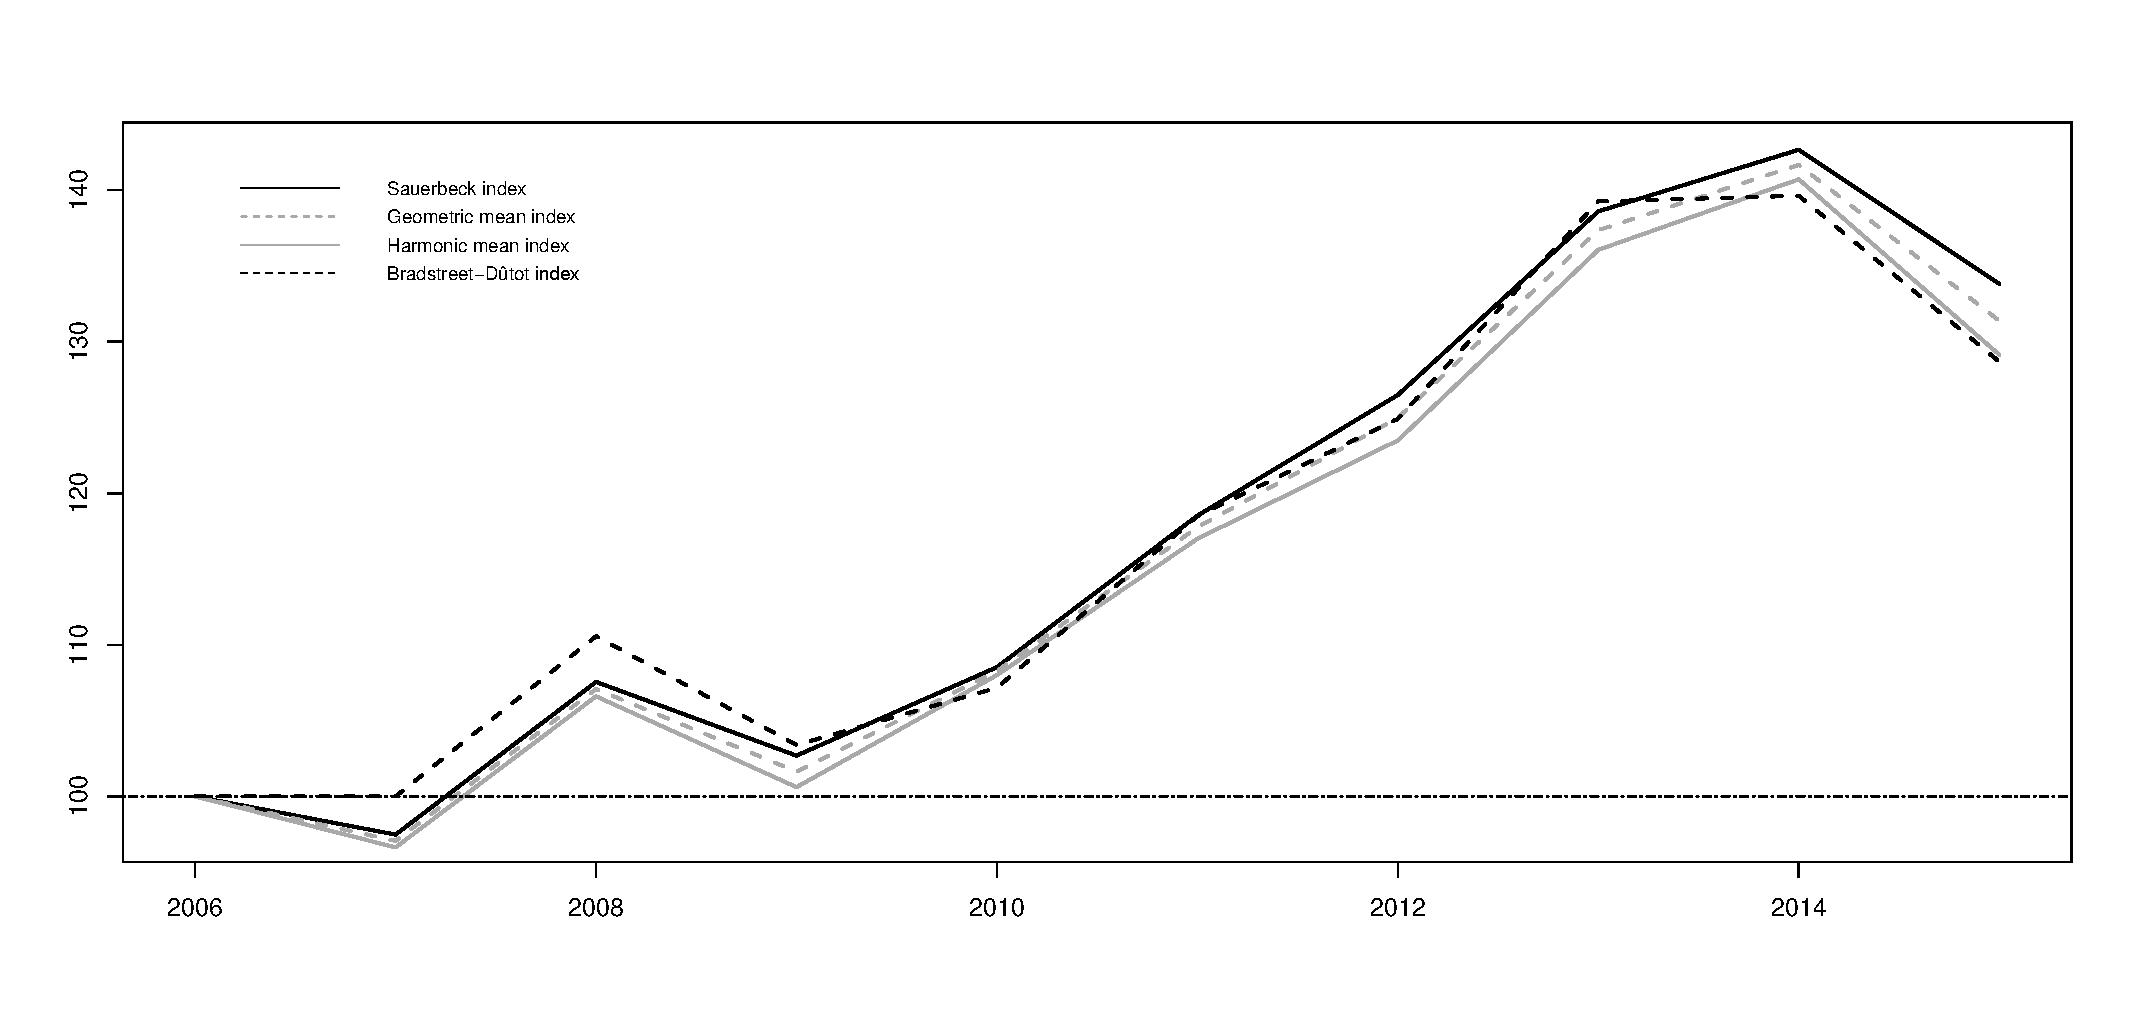
\includegraphics[scale=0.415]{1.pdf}
 	\vspace*{-0.5 cm}\caption{Joint evolution of the non-weighted complex price indexes in series for the unitary value of combustibles and energy resources for the main home in Spain from 2006 to 2015.}
 	\label{nwjointevolution}
 \end{figure}

However,  the variation of a given magnitude in time $t$ with respect to  the previous period may also be  of interest. Below, we alternatively enumerate the mathematical  expressions of the previous indices based on index numbers in chain for the magnitudes.

\begin{itemize}
	\item The \emph{Carli index} (cf. \citealp{carli1804}) at time $t$ for X, $C^t(X)$, is calculated as the arithmetic mean of the simple index in chain for the $n$ involved magnitudes at $t$:
	\begin{equation}\label{niCarli}C^t(X)=\frac{1}{n}\sum_{i=1}^n \frac{x_{it}}{x_{i\mbox{ }t-1}}\cdot 100,\mbox{ for each }t\in\{1,\cdots,T\}.\end{equation}
	\item The \emph{Jevons index} at time $t$, $J^t(X)$, is calculated following \cite{jevons1863serious} as follows:
	\begin{equation}\label{niJevons}J^t(X)=\sqrt[n]{\prod_{i=1}^n \frac{x_{it}}{x_{i\mbox{ }t-1}}}\cdot 100,\mbox{ for each }t\in\{1,\cdots,T\}.\end{equation}
	Given a collection of $n$ magnitudes, the geometric mean index at $t$ is obtained as $n^{th}$-root of the product of simple index numbers for $X$ in chain at time $t$.
%	\item The \emph{Harmonic mean index} at time $t$, $H^t(X)$, is determined by
%	\begin{equation}\label{niHarmonic}H^t(X)=\frac{n}{\sum_{i=1}^n\frac{x_{i0}}{x_{it}}}\cdot 100,\mbox{ for each }t\in\{0,\cdots,T\}.\end{equation}
%	It is initially introduced in \cite{jevons1865variation} and \cite{coggeshall1886arithmetic}.
	\item The \emph{D\^utot index} at time $t$, $D^t(X)$, is introduced in \cite{de1754reflexions}. Its value is obtained as the ratio between the means of the magnitude in time $t$ and the magnitude in time $t-1$ as follows:
	\begin{equation}\label{niDutot}D^t(X)=\frac{\sum_{i=1}^n x_{it}}{\sum_{i=1}^n x_{i\mbox{ }t-1}}\cdot 100,\mbox{ for each }t\in\{1,\cdots,T\}.\end{equation}
\end{itemize}

Again, if $X$ denotes the matrix of prices of a set of goods or services along a period of time ($p$), these index numbers are named as the \emph{Carli index} at time $t$ for prices, $C^t(p)$; the \emph{Jevons index} at time $t$ for prices, $J^t(p)$; and the \emph{D\^utot index} at time $t$ for prices, $D^t(p)$. To conclude this section, we obtain them for the set prices of combustibles and other energy resources for the main home in Spain from 2005 to 2015, detailed in Table \ref{tab1110}. These index numbers are numerically detailed in Table \ref{tab11100002_2}.

\small{
	\begin{table}[h!]\centering\resizebox{0.36\textwidth}{!}{
			\begin{tabular}{|l||ccc|}\hline
				
				$t$	&$C^t(p)$&$J^t(p)$& $D^t(p)$    \\
				
				\hline
		2006&100.00&100.00&100.00\\
		2007&101.11&101.09&101.79\\
		2008&113.51&113.43&115.89\\
		2009&100.94&100.18&126.56\\
		2010&105.75&105.27&144.02\\
		2011&103.58&103.29&155.49\\
		2012&110.65&110.49&168.01\\
		2013&107.00&106.32&163.98\\
		2014&100.72&100.39&154.09\\
		2015&93.08&92.79&153.29\\
				\hline
				%	Simple & & & & & \\   				     	
				%	 indexes  &  178.5714& 148.5714& 122.0000& 111.5942 &108.3333    \\\hline
		\end{tabular}}\caption{Non-weighted complex price indexes in chain for the unitary value of combustibles and energy resources for the main home in Spain from
			2006 to 2015.}\label{tab11100002_2}\end{table}
}

All of the index numbers described are easy to be computed. However, they present an important disadvantage: they do not take into account the relative importance of each product.


\subsubsection{Weighted complex index numbers}

For analyzing the evolution of a given magnitude $X$, it is very common to use an alternative magnitude $Y$ through the value of $Y$ in the reference or the actual period to weight complex index numbers.  The information relative to this alternative variable can be summarized in a table such as Table \ref{0tab111}. For instance,  the use of the amount of production of different products or the use of prices may result of interest, depending on the setting under study.

	\begin{table}[h!]\centering\resizebox{0.45\textwidth}{!}{
		\begin{tabular}{|l||cccc|}\hline
			\backslashbox{Time}{Products} &     $1$&   $2$ &  ... &   $n$ \\\hline
		0  &     $y_{10}$&  $y_{20}$&  ...&  $y_{n0}$\\
		1  &     $y_{11}$&  $y_{21}$&  ...&  $y_{n1}$\\
		$\vdots$  &    $\vdots$&  $\vdots$& $\vdots$&  $\vdots$\\
		$T$  &     $y_{1T}$&  $y_{2T}$&  ...&  $y_{nT}$\\  	
		\hline
	\end{tabular}}\caption{Evolution of a set of magnitudes $Y$ from time $0$ to $T$.}\label{0tab111}\end{table}


Next, the main weighted complex price index numbers for a given magnitude $X$, taking $Y$ as weight, are formally described:
\begin{itemize}
	\item The \emph{Laspeyres index} \citep{laspeyres1871ix} analyzes the variations of $X$ using $Y$ as weight. In this sense, the weights considered for product $i$ are $x_{i0}\cdot y_{i0}$ (note that both values are referred to the base period). Then, this complex index is defined as the weighted arithmetic means of the simple index numbers:
	\begin{equation}\label{niLaspeyres}
L^t(X,Y)=\frac{\sum_{i=1}^n \frac{x_{it}}{x_{i0}}x_{i0}y_{i0}}{\sum_{i=1}^n x_{i0}y_{i0}}\cdot 100 = \frac{\sum_{i=1}^n x_{it}y_{i0}}{\sum_{i=1}^n x_{i0}y_{i0}}\cdot 100,\mbox{ for each }t\in\{0,\cdots,T\}.
	\end{equation}	
	The main disadvantage of the Laspeyres index is that it assumes that the weights do not vary in time. This hypothesis is not always realistic in some practical settings.
	\item The \emph{Paasche index} is an alternative index  to the Laspeyres index introduced in \cite{paasche1874ueber}, when the weighted criteria is $x_{i0}\cdot y_{it}$. Therefore, it can be formally written as:
	\begin{equation}\label{niPaasche}
P^t(X,Y)=\frac{ \sum_{i=1}^n\frac{x_{it}}{x_{i0}}x_{i0}\cdot y_{it} }{\sum_{i=1}^n x_{i0}\cdot y_{it}}\cdot100=  \frac{\sum_{i=1}^n  x_{it}y_{it}}{\sum_{i=1}^n x_{i0}y_{it}}\cdot 100,\mbox{ for each }t\in\{0,\cdots,T\}.
	\end{equation}
	\item The \emph{Marshall-Edgeworth index} (cf. \citealp{marshall1887remedies}, \citealp{edgeworth1887measurement}) is an agregative weighted measure where weights are $y_{i0}+y_{it}$. Therefore, it can be calculated as:
	\begin{equation}\label{niEdgeworth}
E^t(X,Y)=\frac{\sum_{i=1}^n x_{it}(y_{i0}+y_{it})}{\sum_{i=1}^n x_{i0}(y_{i0}+y_{it}) }\cdot 100,\mbox{ for each }t\in\{0,\cdots,T\}.
	\end{equation}
	\item The \emph{Fisher index} is equal to the geometric mean of the index numbers under the approaches of Laspeyres and Paasche:
	\begin{equation}\label{niFisher}F^t(X,Y)=\sqrt{L^t(X,Y)\cdot P^t(X,Y)},\mbox{ for each }t\in\{0,\cdots,T\}.\end{equation}
	For instance, see more details in \cite{fisher1922making}.
	
\end{itemize}




Note that other values can be defined (as we will see below). The choice of using a specific index formula often relies on the availability of data. According to the previous comments, the Laspeyres index does not require information on the products of the current period. Then, the Laspeyres formula is usually preferred for the calculation of complex indices, which are typically released rapidly before information for the current period could have been collected.




In what follows,  $p$ denotes the matrix of prices of a set of goods or services along a period of time and $q$ is the matrix of the total amounts of goods in the same period. Thus, the \emph{weighted complex price index numbers} analyze the time evolution of prices by introducing the variation of the physical production or the consumption of a set of goods or services.  The weights are obtained by multiplying the price of a product in an instant of time $t$ by the consumption in the base period or the actual period. Hence, the \emph{Laspeyres price index}, $L^t(p,q)$, the \emph{Paasche price index}, $P^t(p,q)$, the \emph{Marshall-Edgeworth price index}, $E^t(p,q)$, and the \emph{Fisher price index}, $F^t(p,q)$, are naturally defined in prices settings.



%\vspace*{0.2 cm}\noindent\textbf{Weighted complex price indexes}
%
%\noindent Weighted complex price indexes analyze the time evolution of prices by introducing the variation of the physical production or the consumed amount of a set of goods or services. They can be obtained in a similar way to complex price indexes.  The weighs are obtained multiplying the price of a product in an instant of time $t$ by the consumed amount in the base period or the actual period. 
%
%Next, some weighted complex price indexes are formally decribed. 
%
%\begin{itemize}
%\item 	The \emph{Laspeyres price index} use as weights the values $p_{j0}\cdot q_{j0}$, for each $j=1,\dots,n$ (refered always to the base period). Formally, this price index is given by:
%$$L^t(p,q)=\frac{\sum_{i=1}^n \frac{p_{it}}{p_{i0}}p_{i0}q_{i0}}{\sum_{i=1}^n p_{i0}q_{i0}}\cdot 100 = \frac{\sum_{i=1}^n p_{it}q_{i0}}{\sum_{i=1}^n p_{i0}q_{i0}}\cdot 100,\mbox{ for each }t\in\{0,\cdots,T\}.$$
%
%\item The \emph{Paasche price index} uses the weighted criteria  $p_{i0}\cdot q_{it}$. Therefore, 
%$$P^t(p,q)=\frac{ \sum_{i=1}^n\frac{p_{it}}{p_{i0}}p_{i0}\cdot q_{it} }{\sum_{i=1}^n p_{i0}\cdot q_{it}}\cdot100=  \frac{\sum_{i=1}^n  p_{it}q_{it}}{\sum_{i=1}^n p_{i0}q_{it}}\cdot 100,\mbox{ for each }t\in\{0,\cdots,T\}.$$
%
%\item The \emph{Edgeworth price index} use as weights  $q_{i0}+q_{it}$. Hence,
%$$E^t(p,q)=\frac{\sum_{i=1}^n p_{it}(q_{i0}+q_{it})}{\sum_{i=1}^n p_{i0}(q_{i0}+q_{it}) }\cdot 100,\mbox{ for each }t\in\{0,\cdots,T\}.$$
%
%\item The \emph{Fisher price index} is given by:
%$$F^t(p,q)=\sqrt{L^t(p,q)\cdot P^t(p,q)},\mbox{ for each }t\in\{0,\cdots,T\}.$$
%
%\end{itemize}
%
%
%

Under this approach, a new complex index for $v$ can be naturally introduced under the approach of the {Bradstreet-D\^utot index}. It is based on the notion of the value of good indicated by $v$. It can be calculated as follows:
\begin{equation}\label{nivalue}IV_{0}^t(p,q)=\frac{V_t(p,q)}{V_0(p,q)}=\frac{\sum_{i=1}^n p_{it}q_{it}   }{\sum_{i=1}^n p_{i0}q_{i0} },\mbox{ for each }t\in\{0,\cdots,T\}.\end{equation}
It satisfies that $IV_{0}^t(p,q)=L^t(p_0,q)\cdot P^t(p_0,q)=L^t(p,q_0)\cdot P^t(p,q_0)=F^t(p_0,q)\cdot F^t(p,q_0)$.

%The choice of an index formula often rely on the availability of data. According to the previous comments, the Laspeyres index does not require information on the products of the current period. Then, the Laspeyres formula is usually preferred for the calculation of consumer price indices, which are typically released rapidly before consumption for the current period could have been collected.
%
%   
%
From data contained in Tables \ref{tab1110} and \ref{tab671110}, these five index numbers were determined. They are in Table \ref{tab1110000b} (from 
tenth to twelfth column), and they are graphically depicted in Figure \ref{wjointevolution}.

  \small{
	\begin{table}[h!]\centering\resizebox{0.63\textwidth}{!}{
		\begin{tabular}{|l||ccccc|}\hline
			
			$t$	&$L^t(p,q)$&$P^t(p,q)$& $E^t(p,q)$ &$F^t(p,q)$ & $IV_0^t(p,q)$   \\
			
			\hline
2006 &100.00& 100.00& 100.00& 100.00& 100.00 \\
2007 &101.31& 100.99& 101.15& 101.15& 101.79\\
2008 &110.23& 109.89& 110.06& 110.06& 115.89\\
2009 &112.11& 112.06& 112.09& 112.09& 126.56\\
2010 &115.76& 116.69& 116.27& 116.22& 144.02\\
2011 &127.77& 128.35& 128.08& 128.06& 155.49\\
2012 &142.72& 143.32& 143.04& 143.02& 168.01\\
2013 &153.98& 154.43& 154.21& 154.20& 163.98\\
2014 &158.54& 158.62& 158.58& 158.58& 154.09\\
2015 &158.20& 158.23& 158.21& 158.21& 153.29\\
			\hline
			%	Simple & & & & & \\   				     	
			%	 indexes  &  178.5714& 148.5714& 122.0000& 111.5942 &108.3333    \\\hline
		\end{tabular}}\caption{Weighted complex price indexes for the unitary value of combustibles and energy resources
	 for the main home in Spain from
			2006 to 2015.}\label{tab1110000b}\end{table}\vspace{-0.2 cm}
}


\begin{figure}[htbp]
	\centering
	\hspace*{-0.7 cm}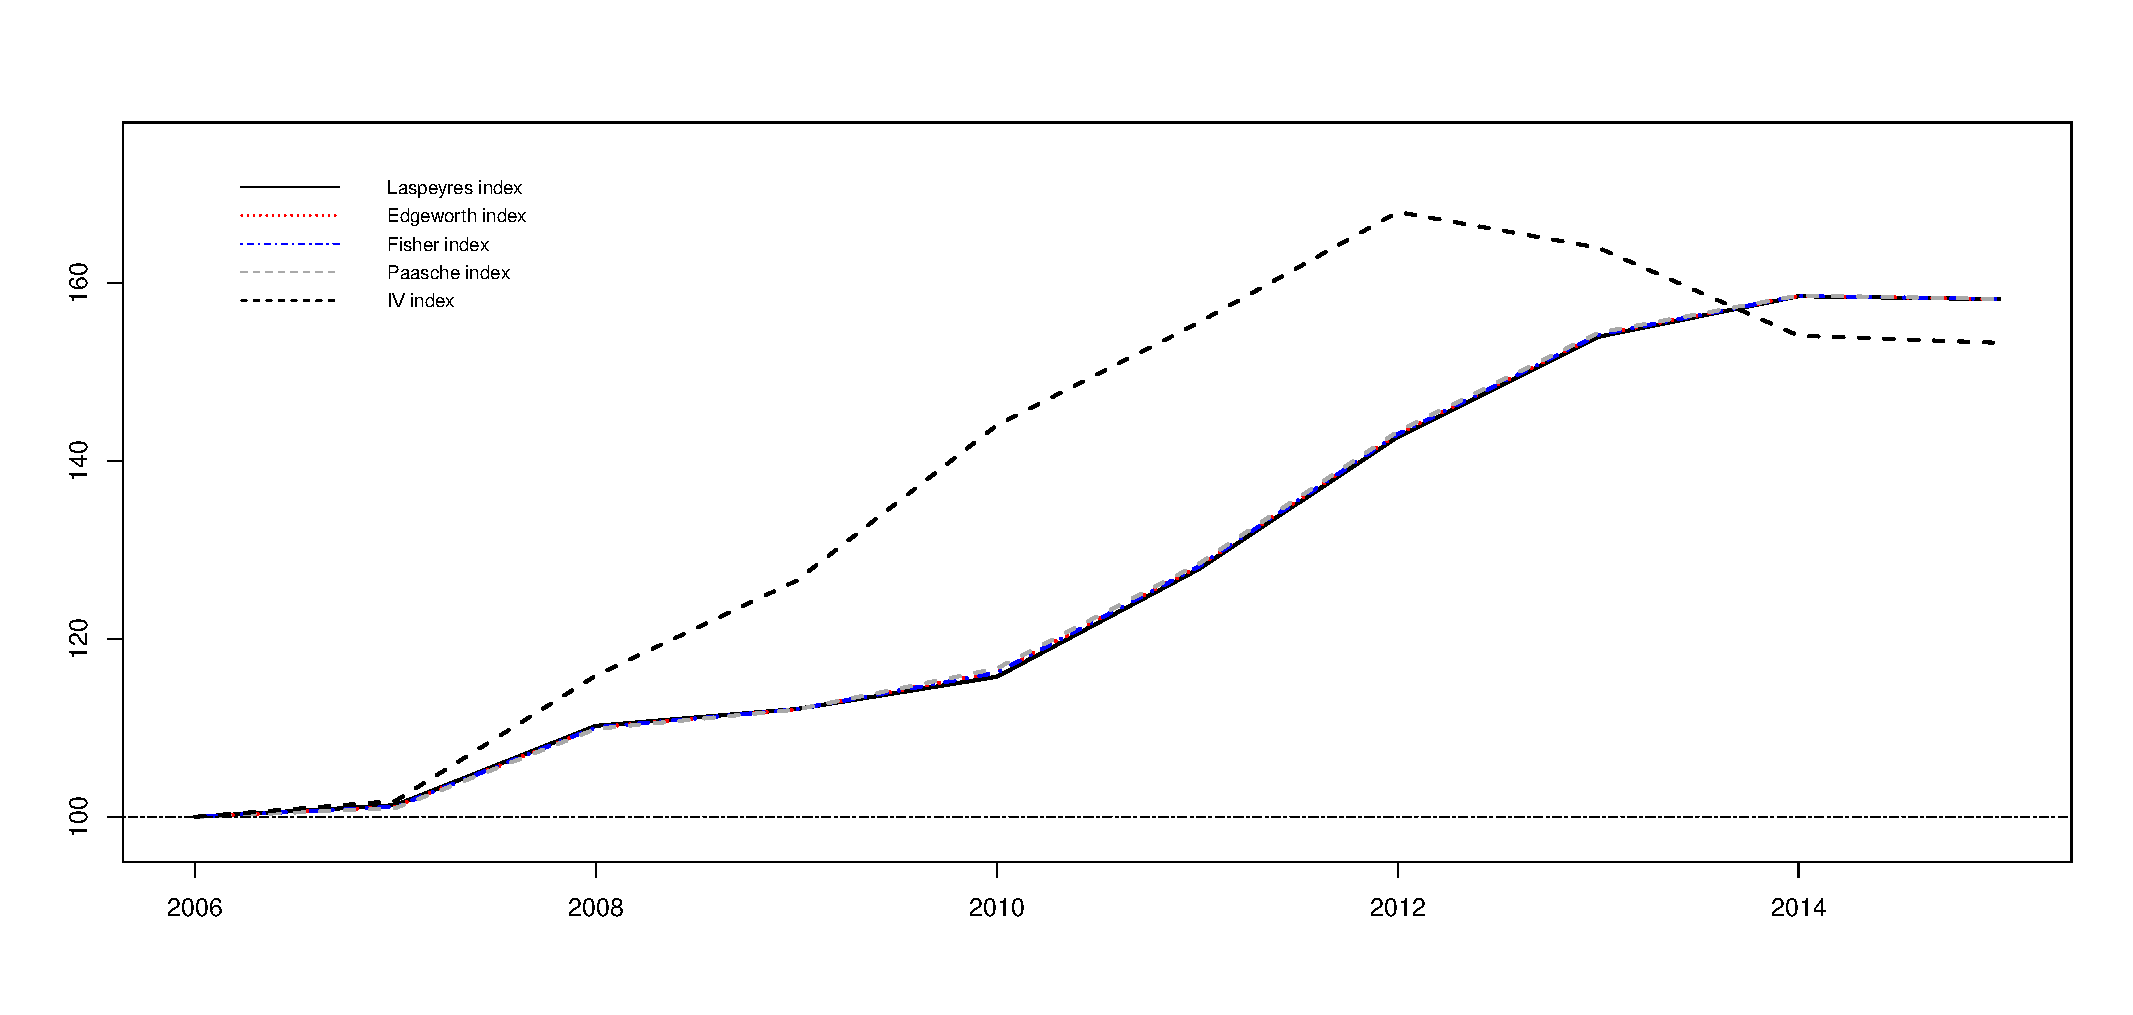
\includegraphics[scale=0.415]{2.pdf}
	\vspace*{-1 cm}\caption{Joint evolution of the weighted complex price indexes for the unitary value of combustibles and energy resources for the main home in Spain from 2006 to 2015.}
	\label{wjointevolution}
\end{figure}\vspace{-0.15 cm}

Otherwise, the \emph{weighted complex production index numbers} analyze the time evolution of the amount of product by introducing the variation of the price of the goods or services as weight. Their obtaining is analogous to the previous one.  The weights are obtained by multiplying the amount of a product in an instant of time $t$ by the prince in the base period or the actual period. Thus, we dealt with the \emph{Laspeyres production index}, $L^t(q,p)$; the \emph{Paasche production index}, $P^t(q,p)$; or the \emph{Fisher production index} $F^t(q,p)$.
%
%
%\vspace*{0.2 cm}\noindent\textbf{Weighted complex production indexes}
%
%\noindent Weighted complex production indexes analyze the time evolution of the amount of product by introducing the variation of the price of the goods or services as weight. Their obtaining is analogous to the previous one.  The weighs are obtained multiplying the amount of a product in an instant of time $t$ by the prince in the base period or the actual period. 
%
% Next, they are formally formalized. 
%
%\begin{itemize}
%\item The \emph{Laspeyres production index} can be written as:
%$$L^t(q,p)=\frac{\sum_{i=1}^n \frac{q_{it}}{q_{i0}} q_{i0}\cdot p_{i0} }{\sum_{i=1}^n q_{i0}p_{i0}} \cdot 100=\frac{ \sum_{i=1}^n q_{it}\cdot p_{i0}  }{\sum_{i=1}^n q_{i0}\cdot p_{i0}  }\cdot 100,\mbox{ for each }t\in\{0,\cdots,T\}.$$ 
%\item The alternative given by the \emph{Paasche production index} is  written as:
%$$P^t(q,p)= \frac{\sum_{i=1}^n \frac{q_{it}}{q_{i0}}q_{i0}p_{it}   }{\sum_{i=1}^n q_{i0}p_{it}}\cdot 100=\frac{\sum_{i=1}^n q_{it}\cdot p_{it} }{ \sum_{i=1}^n q_{i0}\cdot p_{it}  }\cdot 100 ,\mbox{ for each }t\in\{0,\cdots,T\}.$$
%\item The \emph{Fisher production index} is given by:
%$$F^t(q,p)=\sqrt{L^t(q,p)\cdot P^t(q,p)},\mbox{ for each }t\in\{0,\cdots,T\}.$$
%\end{itemize}
%%These weighted complex production indexes  are calculated for the data in Tables \ref{tab1110} and \ref{tab671110}. They are depicted in Table \ref{tab1110000}.
%		 

\section{IndexNumber in practice}\label{indexnumberinpractice}\vspace{-0.3 cm}
This section presents an overview of the structure of the package. \pkg{IndexNumber} is a tool that R users can use in order to determine  several classical index numbers that describe the evolution of a single magnitude or a set of magnitudes. This software helps the user to calculate faster these statistical measures. Functions in this library automatize the required operations for the computation of index numbers. First, we will describe the real data sets included in the package. Then, the functions implemented are detailed. Of course, other libraries exist in R dealing with index numbers theory. In particular, \pkg{micEconIndex} \citep{micEconIndex}, \pkg{IndexNumR} \citep{indexnumR}, and \pkg{PriceIndices} \citep{PriceIndices} packages also allow to compute complex index numbers but only when the considered magnitudes are prices and quantities. It is worth mentioning that \pkg{IndexNumber} library was designed under a more general perspective by extending to any type of magnitude. Moreover, none of the above-referenced packages implement simple index numbers, and they do not offer graphical tools to facilitate the analysis of time evolution series either. Additionally, \pkg{IndexNumber} can be seen as an additional basic  library that can also be exploited by non-experts R users. For instance, inputs of functions are numeric vectors or matrices containing the magnitude values, much more flexible than data structures that other packages consider. As for computational complexity, it is also relatively simple because, unlike \pkg{IndexNumR} that implements multilateral methods, the number of required elementary operations is smaller. Finally, it is convenient to note that \pkg{IndexNumber} package also provides four new recent real data sets.\vspace{-0.15 cm}


\subsection{Data sets in IndexNumber}

Index numbers have been theoretically introduced in previous sections using two real data sets included in the package \pkg{IndexNumber}.  However, we decide to include them in the package because they could be used directly by the users, avoiding  search and  download. Besides, two additional data sets were also included. All of them are  available in the website of the Spanish Statistical Office (INE), \url{http://www.ine.es}. These four data sets are briefly described below:\vspace{-0.15 cm}
\begin{itemize}
	\item Firstly, the data set \verb|ActivePeople| was considered as an example in order to illustrate the simple index numbers. It contains information separately on the number (thousands) of economically active women and men in Spain from the first trimester in 2002 to the fourth one in 2019.  

\item Secondly, \verb|ECResources| is a data set containing as variables, the unitary value (euros) and consumption (thousands of units) of several combustibles and other energy resources for the main home in Spain from 2006 to 2015. It was used in this paper for illustrating complex index numbers.

\item An additional data set called \verb|Mortgages| was also included in the package. In this case, the variables correspond to the number of mortgages constituted on urban properties in Spain from 2003 to 2018, distinguished between the kind of mortgages entities (banks, saving banks and other types). The corresponding mortgages amounts (thousands of euros) were also included as variables.

\item Finally, the variables in the data set \verb|Food| are the unitary value (euros) and consumed amount (thousands of units) of the main types of food in Spain from 2006 to 2015. 
\end{itemize}

Once the package is installed and loaded, a full description of these data sets is shown through \verb|help(ActivePeople)|, \verb|help(ECResources)|, \verb|help(Mortgages)|, and \verb|help(Food)|, respectively.

\subsection{Functions in IndexNumber}

\pkg{IndexNumber} package includes several functions that enable users to determine the index numbers, simple and complex (weighted and non-weighted), described in previous sections.  The functions incorporated in the package are summarized in Table \ref{table_summary1}.

\begin{center}\small
	\begin{longtable}{l p{9.7 cm}}
		\toprule
		Function & Description \\\midrule
		\code{aggregated.index.number} & Function to obtain several non-weighted index numbers: the Sauerbeck index number (\ref{niSauerbeck}), the Geometric index number (\ref{niGeometric}), the Harmonic index number (\ref{niHarmonic}) the Bradstreet-Dûtot index number (\ref{niBDutot}), the Carli index number (\ref{niCarli}), the Jevons index number (\ref{niJevons}) and the Dûtot index number in (\ref{niDutot}).  \\
		\code{edgeworth.index.number} & Function to calculate the Marshall-Edgeworth index number (\ref{niEdgeworth}).  \\
		\code{fisher.index.number} & Function to calculate the Fisher index number (\ref{niFisher}).  \\
		\code{index.number.chain} & Function to calculate the simple index number in chain (\ref{niinchain}).  \\
		\code{index.number.serie} & Function to calculate the simple index number in series (\ref{niinserie}). \\
		\code{laspeyres.index.number}& Function to determine the Laspeyres index number (\ref{niLaspeyres}).\\
		\code{paasche.index.number}& Function to obtain the Paasche index number (\ref{niPaasche}).\\
	
		\bottomrule
		%\end{tabular}\end{center}
		\caption{Summary of functions in the \pkg{IndexNumber} package.}\label{table_summary1}
	\end{longtable}
\end{center}



\vspace*{-0.5 cm}Users can obtain different kinds of index numbers by introducing the associated  parameters in the corresponding function.  Table \ref{table2} describes the different options to determine those index numbers whose implementation was included in \pkg{IndexNumber} package. However, not all of the mentioned options are required since  only some of them are specific for each particular class of index number. Thus, Table \ref{table3} summarizes the  arguments associated with  each function. Examples of usage for the implemented functions are described in the next section.



\begin{center}\small
	\begin{longtable}{l p{11.75 cm}}
		\toprule
		Argument & Description \\\midrule
		\code{x} & A matrix that contains the magnitude(s) under study. In each column, it contains the magnitude of a different product considered. Thus, we have \code{nrow(x)} values of a magnitude for \code{ncol(x)} products. Notice that if we intend to analyze a single magnitude, \code{x} corresponds to a vector of length equal to the total instants of time registered.\\	
		\code{y} & A matrix that contains that magnitude used as weight. In each column, it contains another magnitude associated to each different product along the time. Thus, we have \code{nrow(x)} values of  magnitudes for the set of \code{ncol(x)} products. It is only required for obtaining those weighted index numbers mentioned in the paper.\\	
		\code{base} & A chain of characters that indicates the nature of the index number. If we introduce \code{base="serie"}, we compare each value with respect to the initial one. In this case, it is said to be an index number in series. Otherwise, if we introduce \code{base="chain"}, we obtain the index number in chain, by comparing each value with the immediately previous value.\\
		\code{type} & A chain of characters to indicate the type of non-weighted index number to evaluate the evolution of a set of magnitudes (even for different products). \newline By considering \code{base="serie"}, if we introduce \code{type="arithmetic"}, we obtain the Sauerbeck index number in (\ref{niSauerbeck}). If we introduce \code{type="geometric"}, we obtain the Geometric index in (\ref{niGeometric}). If we choose \code{type="harmonic"}, we obtain the Harmonic mean index in (\ref{niHarmonic}). If we write \code{type="BDutot"}, we will obtain the Bradstreet-Dûtot index in (\ref{niBDutot}). This argument is only  required  in the function \code{aggregated.index.number}.
		\newline Otherwise, if we take \code{base="chain"} and \code{type="Carli"}, we obtain the Carli index number in (\ref{niCarli}). If we introduce \code{type="Jevons"}, we obtain the Jevons index in (\ref{niJevons}) and if we choose \code{type="Dutot"}, we obtain the Dûtot index in (\ref{niDutot}). \newline
		This argument is only  required  in the function \code{aggregated.index.number}.\\
		\code{name} & A chain of characters to indicate the name of the variable under study.\\
		\code{opt.plot}& A Boolean variable that indicates if a graphical description of the index number along the different stages is required. If it is desired, \code{opt.plot=TRUE}, else \code{opt.plot=FALSE}.\\
		\code{opt.summary}& A Boolean variable that indicates if a basic statistical summary of the index number is required. If it is desired, \code{opt.summary=TRUE}, else \code{opt.summary=FALSE}.\\
%		   & \\
%		\code{x} &A character string that indicates the selected model and required only in the \code{inventorymodelfunction}. The possible values are \code{"EOQ"} (EOQ), \code{"EPQ"} (EPQ), \code{"STI"} (the inventory transportation systems), \code{"FOC"} (the fixed order cost model), \code{"MCT"} (the basic EOQ system without holding costs and with
%		transportation cost), \code{"MWHC"} (the model without holding costs and shortages), \code{"MWHC2"} (the model without holding costs and two acquisition costs) and \code{"MWHCCT"} (the EOQ system without holding costs and with general transportation costs).\\
%		\code{n} & An integer specifying the number of agents involved in the inventory model. It corresponds to the cardinality of the set $N$.\\
%		\code{a}& A real number that indicates the fixed cost per new order.\\
%		\code{av}& A vector of dimension \code{n} that contains, in each component, the transportation costs associated with each agent $i\in N$.\\
%		\code{d}& A vector of dimension \code{n} that contains, in each component, the deterministic demands per time unit associated with each agent $i\in N$.\\
%		\code{h}& A vector of dimension \code{n} that indicates, in each component, the holding costs per product unit associated with each agent $i\in N$.\\
%		\code{m}& A vector of dimension \code{n} that indicates, in each component, the number of orders $m_i$ associated with each agent $i\in N$. These values are necessary only when information about demands is unknown.\\
%		\code{r}& A vector of dimension \code{n} that contains, in each component, the replacement rate of a product associated with each agent $i\in N$ in a EPQ model. In general, it verifies $r_i>d_i$.\\
%		\code{K}& A vector of dimension \code{n} that details, in each component, the warehouse capacity of the product associated with each agent $i\in N$.\\
%		\code{b}&  A vector of dimension \code{n} that details, in each component, the cost by shortage unit of the product associated with each agent $i\in N$.\\
%		\code{c1}& A real value with the {acquisition cost} of one unit of the {purchased} commodity.\\
%		\code{c2}& A real value with the {acquisition cost} of one unit of the {produced} commodity.\\
%		\code{cooperation}& A Boolean variable that indicates if cooperation is considered. If it exists, \code{cooperation=1}, else \code{cooperation=0}.\\
%		\code{allocation}& A Boolean variable that indicates if the defined allocation in each case is required. If it exists, \code{allocation=1}, else \code{allocation=0}.\\
		\bottomrule\caption{Summary of arguments for functions in the \pkg{IndexNumber} package.}\label{table2}
	\end{longtable}
\end{center}


\vspace*{-0.6 cm}\begin{table}[h]\begin{center}\resizebox{0.8\textwidth}{!}{\begin{tabular}{lccccccc}
				\toprule
				Function & \code{x} & \code{y}& \code{base}& \code{type}& \code{name}& \code{opt.plot}& \code{opt.summary}\\\midrule
				%\code{coalitions} &- & \checkmark & -& -& -& -& -& -& -& -& -& -& -& -& -\\
				\code{aggregated.index.number} &  \checkmark&- & \checkmark& \checkmark& \checkmark& \checkmark& \checkmark\\
	\code{edgeworth.index.number} &  \checkmark&\checkmark & -& -& \checkmark& \checkmark& \checkmark\\
	\code{fisher.index.number} &  \checkmark&\checkmark & -& -& \checkmark& \checkmark& \checkmark\\
	\code{index.number.chain} &  \checkmark&- & -& -& \checkmark& \checkmark& \checkmark\\
	\code{index.number.serie} &  \checkmark&- & -& -& \checkmark& \checkmark& \checkmark\\
\code{laspeyres.index.number} &  \checkmark&\checkmark & -& -& \checkmark& \checkmark& \checkmark\\
\code{paasche.index.number} &  \checkmark&\checkmark & -& -& \checkmark& \checkmark& \checkmark\\
%				\code{EOQcoo} &  - & \checkmark& \checkmark& -& \checkmark& \checkmark& \checkmark& -& -& -& -& -&  -& -\\
%				\code{EPQ} & -& \checkmark&\checkmark& -& \checkmark& \checkmark&\checkmark& \checkmark& -&\checkmark& -& -& -& -\\
%				\code{EPQcoo} & -& \checkmark&\checkmark& -& \checkmark& \checkmark& \checkmark& \checkmark&-&\checkmark& -& -& -& -\\
%				\code{inventorygames}& \checkmark & -& \checkmark& -& \checkmark& \checkmark&\checkmark& \checkmark& -&\checkmark& -& -& -& -\\
%				\code{inventorymodelfunction}&\checkmark & \checkmark& \checkmark& \checkmark& \checkmark& \checkmark& \checkmark& \checkmark& \checkmark& \checkmark& \checkmark& \checkmark& \checkmark& \checkmark\\
%				\code{linerule} & - & \checkmark&\checkmark& \checkmark& \checkmark& \checkmark& \checkmark& -& -&-& -& -&  -& -\\
%				\code{linerulecoalitional} & - &\checkmark&\checkmark& \checkmark& \checkmark& \checkmark& \checkmark& -& -&-&  -& -& -& -\\
%				\code{mct}& - & \checkmark& \checkmark& \checkmark& \checkmark& -& -&  -& \checkmark& -& -& -& \checkmark& -\\
%				\code{mfoc}& - & \checkmark& \checkmark&-& \checkmark& -& -& -& \checkmark& -& -& -& \checkmark& -\\
%				\code{mwhc}& - & \checkmark& \checkmark& -& \checkmark&-& -& -&  \checkmark& \checkmark& -& -& \checkmark& \checkmark\\
%				\code{mwhc2c}& - & \checkmark& \checkmark& -& \checkmark&-&-& -& \checkmark& \checkmark& \checkmark& \checkmark& \checkmark& \checkmark\\
%				\code{mwhcct} & - & \checkmark& \checkmark& \checkmark& \checkmark& -& -& -&  \checkmark& -& -& -& \checkmark& \checkmark\\
%				\code{shapley\_mfoc}& - &\checkmark& \checkmark&-& \checkmark& -& -& -& \checkmark& -& -& -& -& -\\
%				\code{SOC}& \checkmark & \checkmark& \checkmark& -& \checkmark& \checkmark& \checkmark&\checkmark& -& -& -&  -& -& -\\
%				\code{STI}& - & \checkmark& \checkmark& \checkmark& \checkmark& \checkmark& \checkmark& -& -& -& -& -& -& -\\
%				\code{STIcoo}& - & \checkmark& \checkmark& \checkmark& \checkmark& \checkmark&\checkmark& -& -& -& -& -& -&  -\\
%				\code{twolines}& - & \checkmark& \checkmark& \checkmark& \checkmark& -&  -& -& \checkmark& -&-& -& -& -\\		
%				
				\bottomrule
		\end{tabular}}\vspace{-2 mm}\end{center}\caption{Arguments for each function in the \pkg{IndexNumber} package.}\label{table3}\end{table}


\subsection{Examples of using IndexNumber}
In what follows, we describe several examples of the application of the \pkg{IndexNumber} package that is used to illustrate its performance. Initially,  a  user has to incorporate the package from the CRAN in the R Console. After its installation, the next code allows its usage:
\begin{example}
> library("IndexNumber")
\end{example}
Below, it is shown how to use the different functions implemented for determining index numbers on the real data sets presented in the preliminaries section.

\subsubsection{Simple index numbers in series in R}

The example that we consider describes the obtaining of the simple index numbers  in series (\ref{niinserie}) in R software on the real data partially given in Table \ref{tab0}. Remember that it depicts the number (thousands) of economically active women and men in Spain. As we mentioned before, this information is also included in the data set \verb|ActivePeople| in \pkg{IndexNumber} package. The first trimester of 2002  is considered as the reference value. 

Using \verb|index.numer.serie()| function, we obtain the simple index number in series for the first instants of time  in the example. 

\begin{example}
> index.number.serie(ActivePeople$TotalWomen[1:15],name="Woman",opt.plot=TRUE,
                     opt.summary = TRUE)
                     
Index number in serie

Summary

Min.=101.855509425343

Stage=1

Max.=117.978690528975

Stage=13

$Summary
 Min. 1st Qu.  Median    Mean 3rd Qu.    Max. 
101.9   106.1   110.4   110.3   114.6   118.0 

$`Index number`
   Stages  Woman Index number
1       0 7442.7     100.0000
2       1 7580.8     101.8555
3       2 7670.2     103.0567
4       3 7751.5     104.1490
5       4 7868.7     105.7237
6       5 7977.8     107.1896
7       6 8093.3     108.7415
8       7 8190.9     110.0528
9       8 8249.7     110.8428
10      9 8348.9     112.1757
11     10 8430.8     113.2761
12     11 8564.6     115.0738
13     12 8635.2     116.0224
14     13 8780.8     117.9787
15     14 8769.1     117.8215
\end{example}

We include a graphical summary of the evolution of this magnitude under the fixed criteria in Figure \ref{women_in_serie}, by using \verb|opt.plot=TRUE|. We also summarize the most relevant information in terms of the instant in which the maximum and minimum values are reached choosing \verb|opt.summary=TRUE|.

\begin{figure}[h!]
	\centering
	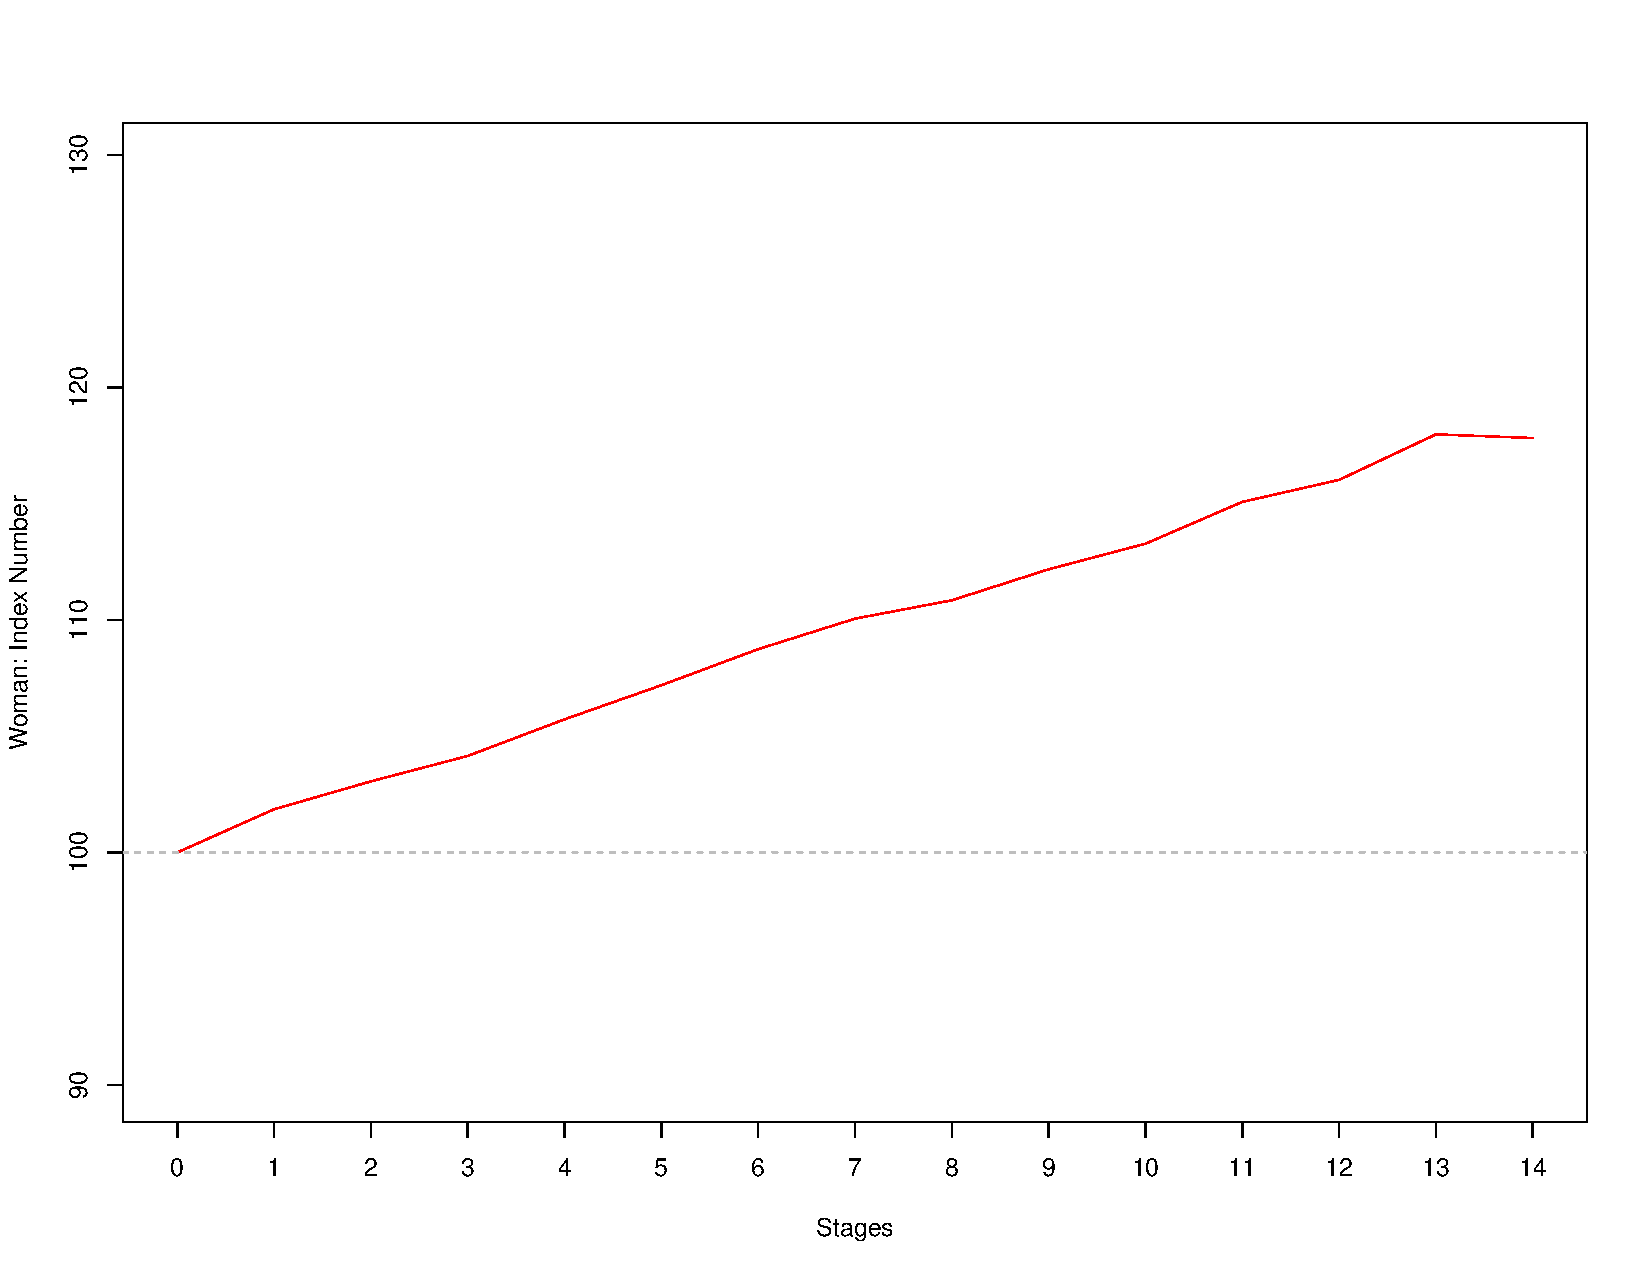
\includegraphics[scale=0.4]{inseriewoman_new.pdf}
	\caption{Evolution of the simple index number in series for the number (thousands)  of economically active women in Spain.}
	\label{women_in_serie}
\end{figure}





Analogously, the user can obtain the corresponding results for the data associated to \verb|TotalMen|. The required code in this case is the shown below:
\begin{example}
index.number.serie(ActivePeople$TotalMen[1:15],name="Man",opt.plot=TRUE,opt.summary = TRUE)
\end{example}

Results contained in Table \ref{tab1} have been obtained using both functions of \pkg{IndexNumber} package in R.

\subsubsection{Simple index numbers in chain in R}

Again, we take the data set \verb|ActivePeople| to determine the corresponding simple index number in chain (\ref{niinchain}) for the number (thousands) of economically active women in Spain. Note that the reference value in each instant of time is the immediately previous one in the series. 

Alternatively, we use \verb|index.numer.chain()| function for obtaining the simple index number in chain for the first instants of time for the variable considered in the example. 

\begin{example}
> index.number.chain(ActivePeople$TotalWomen[1:15],name="Woman",opt.plot=TRUE,
                     opt.summary = TRUE)
                     
Index number in chain

Summary

Min.=99.8667547376093

Stage=14

Max.=101.855509425343

Stage=2

$Summary
 Min. 1st Qu.  Median    Mean 3rd Qu.    Max. 
99.87  101.00  101.20  101.18  101.50  101.86 

$`Index number`
   Stages  Woman Index number
1       0 7442.7    100.00000
2       1 7580.8    101.85551
3       2 7670.2    101.17930
4       3 7751.5    101.05995
5       4 7868.7    101.51197
6       5 7977.8    101.38651
7       6 8093.3    101.44777
8       7 8190.9    101.20594
9       8 8249.7    100.71787
10      9 8348.9    101.20247
11     10 8430.8    100.98097
12     11 8564.6    101.58704
13     12 8635.2    100.82432
14     13 8780.8    101.68612
15     14 8769.1     99.86675
\end{example}

Also in this case, the option \verb|opt.summary=TRUE| summarizes the most relevant information about the corresponding simple index number. The option \verb|opt.plot=TRUE| provides a graphical representation of the evolution of the magnitude as Figure \ref{women_in_chain} depicts. 

\begin{figure}[htbp]
	\centering
	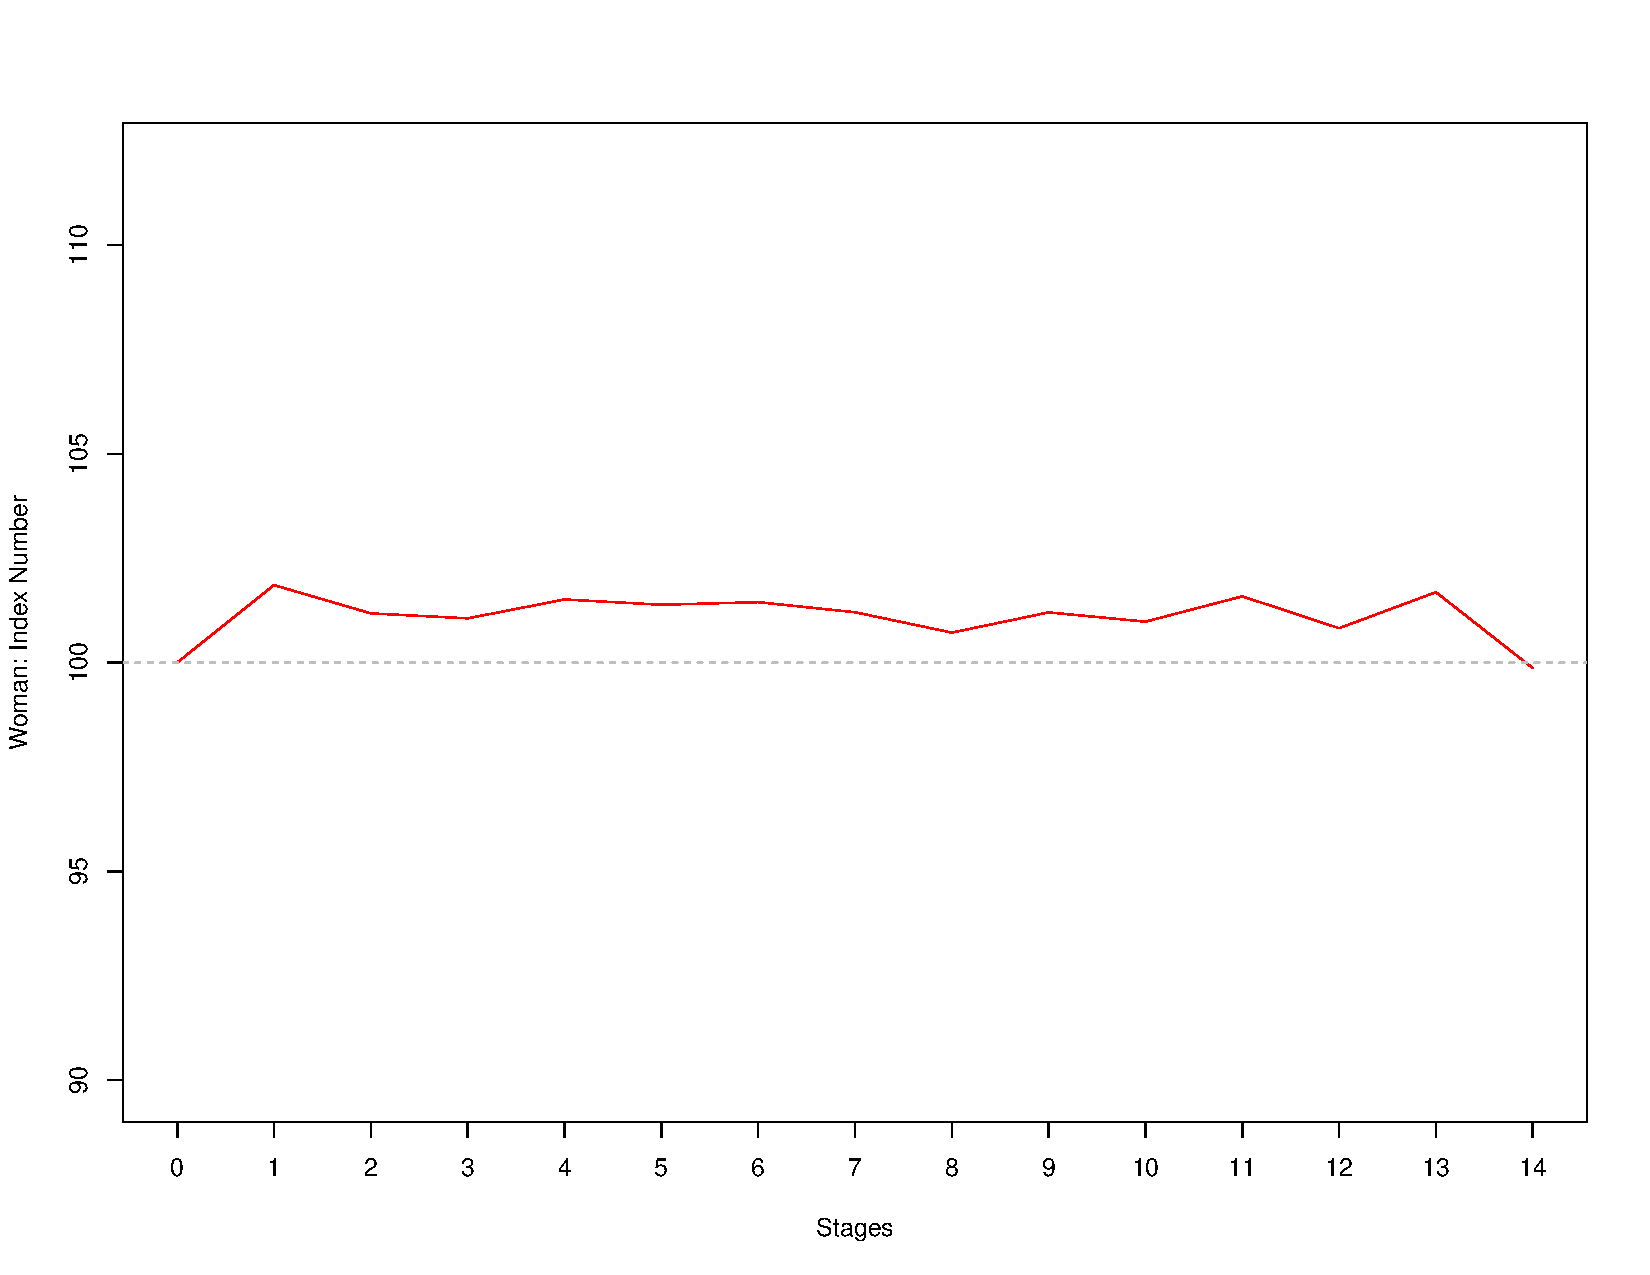
\includegraphics[scale=0.4]{inchainwomen_new.pdf}
	\caption{Evolution of the simple index number in chain for the number (thousands) of economically active women in Spain.}
	\label{women_in_chain}
\end{figure}

Table \ref{tab4} also includes the numerical analysis of the evolution of  economically active men in Spain. To determine these values, we use the following code:
\begin{example}
index.number.chain(ActivePeople$TotalMen[1:15],name="Man",opt.plot=TRUE,opt.summary = TRUE)
\end{example}


\subsubsection{Non-weighted complex index numbers in R}

In this section, we illustrate the usage of \pkg{IndexNumber} to determine non-weighted complex index numbers. 

As in its theoretical description, we take the example described in Table \ref{tab1110} to show its performance in practice. That table describes the unitary value of prices of several energy resources for the period 2005-2015. As we have mentioned, this data set is available in library \pkg{IndexNumber} under the name \verb|ECResources| (in particular, from the second to the sixth column).
\begin{example}[fontsize=\footnotesize]
> ECResources[,2:6]
   ElectricityPrice NaturalGasPrice LiquifiedGasPrice LiquifiedCombustiblesPrice SolidCombustiblesPrice
1              0.14            0.70              1.00                       0.69                   0.12
2              0.14            0.78              0.97                       0.66                   0.10
3              0.15            0.83              1.03                       0.81                   0.11
4              0.16            0.87              0.93                       0.68                   0.10
5              0.17            0.79              1.04                       0.72                   0.12
6              0.19            0.77              1.15                       0.91                   0.12
7              0.22            0.82              1.19                       0.96                   0.12
8              0.23            1.00              1.34                       0.99                   0.13
9              0.24            1.07              1.35                       0.89                   0.15
10             0.25            1.04              1.22                       0.77                   0.13
\end{example}

\vspace*{0.5 cm}First, we describe the R procedures that provide the variations of a magnitude in time $t$ with respect to the base period by using non-weighted index numbers. For this purpose, we have to introduce the option \verb|base="serie"|. Notice that all the values included in Table \ref{tab1110000} were obtained by using the code in R that we show in the current section.

\vspace*{0.15 cm}\noindent\textbf{Sauerbeck index in R}

\noindent Next, we determine the Sauerbeck index (\ref{niSauerbeck}) in R software. To this aim, we use the corresponding function \verb|aggregated.index.number()| by adding, as option, \verb|type="arithmetic"|. Recall that it corresponds to an average by stages. In this case, we also include a graphical description of the joint evolution of prices in Figure \ref{sauerbeck} with \verb|opt.plot=TRUE|, and a numerical summary of such magnitude (with \verb|opt.summary=TRUE|).

\begin{figure}[htbp]
	\centering
	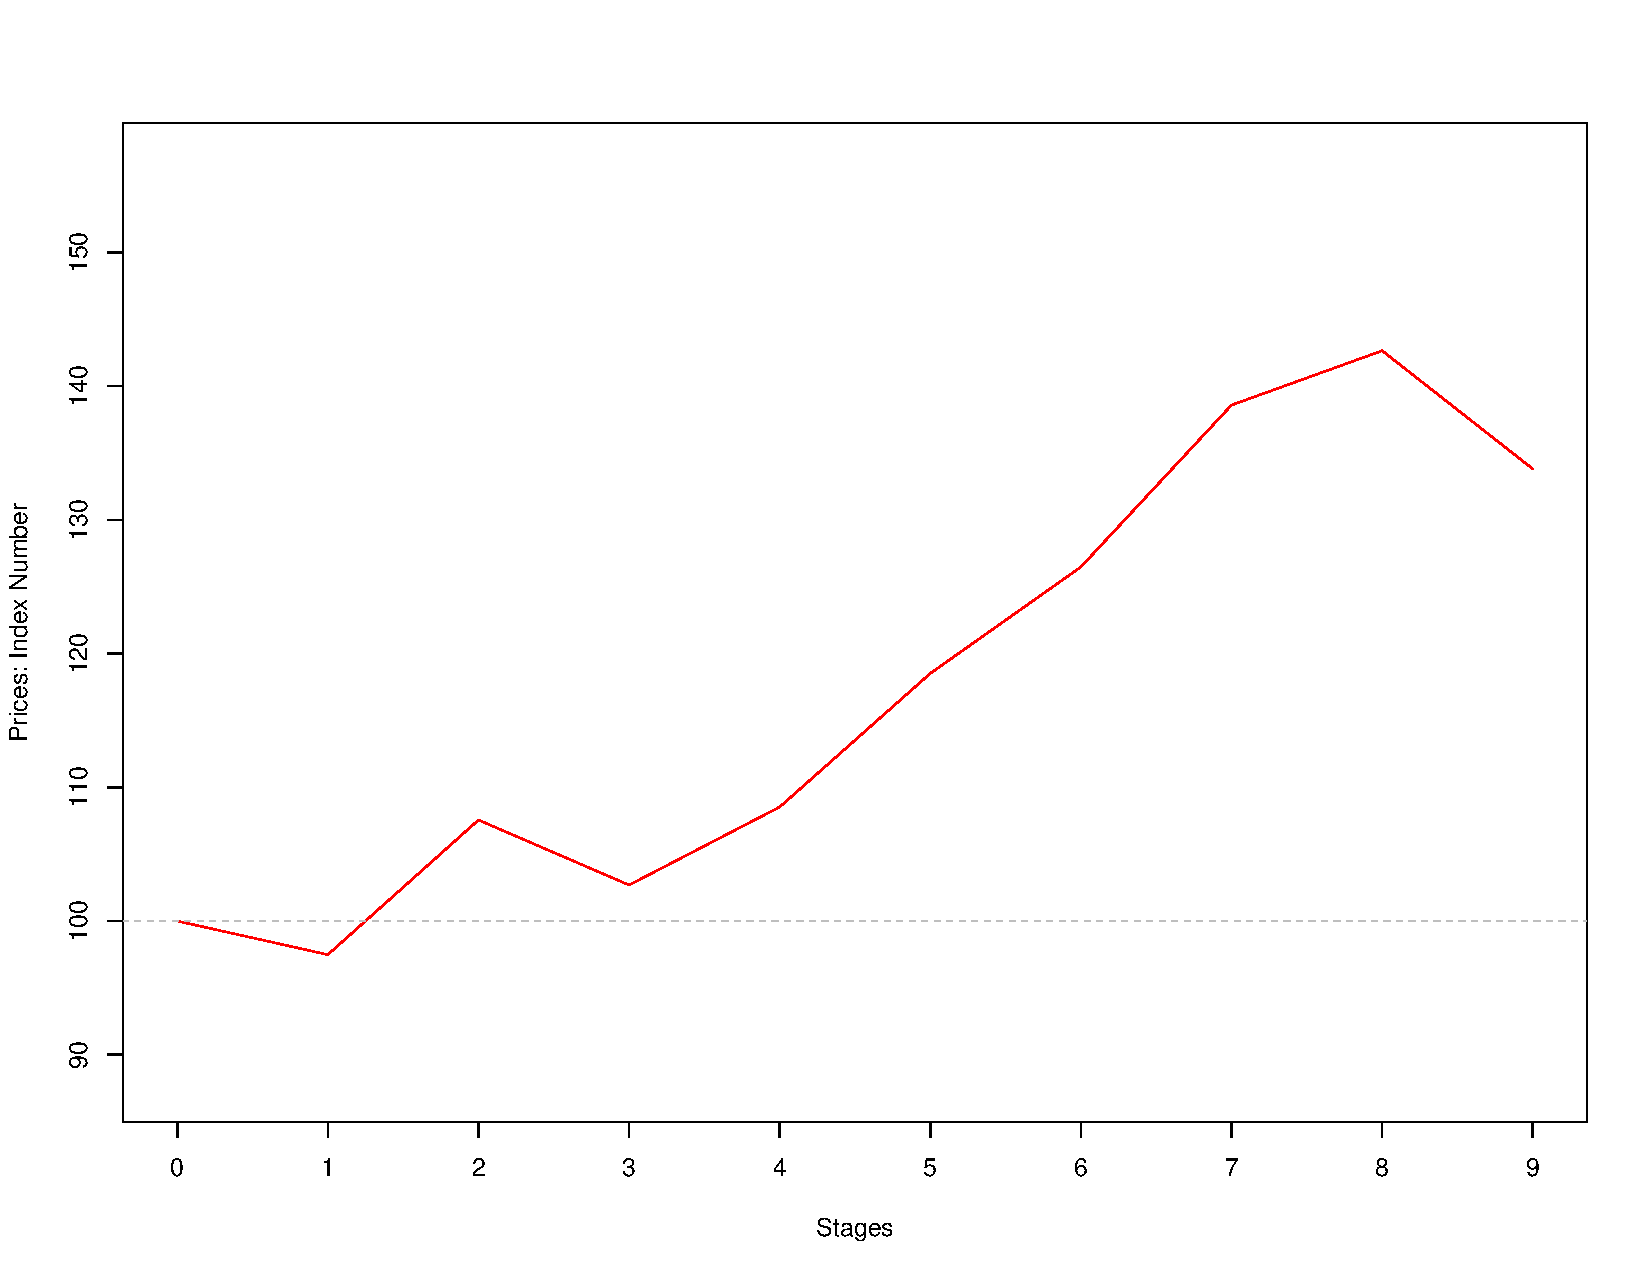
\includegraphics[scale=0.4]{sauerbeck_new.pdf}
	\caption{Sauerbeck index evolution for the prices of several energy resources for the period 2005-2015.}
	\label{sauerbeck}
\end{figure}

\begin{example}
> aggregated.index.number(ECResources[,2:6],base="serie",type="arithmetic",
                          name="Prices",opt.plot=TRUE,opt.summary=TRUE)

Aggregate index number

Arithmetic

Summary

Min.=97.4828157349897

Stage=1

Max.=142.654244306418

Stage=8

$Summary
 Min. 1st Qu.  Median    Mean 3rd Qu.    Max. 
97.48  107.55  118.52  119.59  133.81  142.65 

$`Agg. index number`
   Stages Prices 1 Prices 2 Prices 3 Prices 4 Prices 5 Agg. index number
1       0     0.14     0.70     1.00     0.69     0.12         100.00000
2       1     0.14     0.78     0.97     0.66     0.10          97.48282
3       2     0.15     0.83     1.03     0.81     0.11         107.55445
4       3     0.16     0.87     0.93     0.68     0.10         102.69110
5       4     0.17     0.79     1.04     0.72     0.12         108.52671
6       5     0.19     0.77     1.15     0.91     0.12         118.51967
7       6     0.22     0.82     1.19     0.96     0.12         126.48323
8       7     0.23     1.00     1.34     0.99     0.13         138.59089
9       8     0.24     1.07     1.35     0.89     0.15         142.65424
10      9     0.25     1.04     1.22     0.77     0.13         133.81408
\end{example}



\vspace*{0.15 cm}\noindent\textbf{Geometric mean index in R}

\noindent The second approach that we consider is the one given by the Geometric mean index (\ref{niGeometric}).  To obtain for the case of prices of the energetic resources, we slightly change the parameters of the function \verb|aggregated.index.number()|. We have to introduce the parameter \verb|type="geometric"| on it. 
\begin{example}
aggregated.index.number(ECResources[,2:6],base="serie",type="geometric",
                        name="Prices",opt.plot=FALSE,opt.summary=FALSE)
\end{example}
The results have the same structure as the previous case that we have explained. For this reason, they have not already been included here.

\vspace*{0.15 cm}\noindent\textbf{Harmonic mean index in R}

\noindent The third option of a non-weighted complex index is the Harmonic mean index (\ref{niHarmonic}). With regard to the previous cases, the main difference is the parameter \verb|type| that, in this case, has to take the value \verb|"harmonic"|.
\begin{example}
aggregated.index.number(ECResources[,2:6],base="serie",type="harmonic",
                        name="Prices",opt.plot=FALSE,opt.summary=FALSE)
\end{example}
The scheme of showing the results maintains also in this scenario.


\vspace*{0.15 cm}\noindent\textbf{Bradstreet-D\^utot index in R}

\noindent The Bradstreet-D\^utot index (\ref{niBDutot}) is determined in R software by using  \verb|aggregated.index.number()| with the parameter \verb|type="BDutot"|. We illustrate the case of obtaining the indicated index for the prices of energetic resources. Again, the output has the same structure as the previous cases.

\begin{example}
aggregated.index.number(ECResources[,2:6],base="serie",type="BDutot",
                        name="Prices",opt.plot=FALSE,opt.summary=FALSE)
\end{example}

\vspace*{0.5 cm}Secondly, we describe examples of usage of \pkg{IndexNumber} package that involves non-weighted and weighted index numbers in chain. Specifically, we show those ones required for obtaining the results in Table \ref{tab11100002_2}. They involves the usage of  \verb|base="chain"|. 

\vspace*{0.15 cm}\noindent\textbf{Carli index in R}

\noindent The Carli index (\ref{niCarli}) is obtained in R software through  \verb|aggregated.index.number()| with \verb|type="Carli"|. The following R code determines the indicated index for the prices of energetic resources with an analogous structure for the output.
\begin{example}
aggregated.index.number(ECResources[,2:6],base="chain",type="Carli",
			name="Prices",opt.plot=FALSE,opt.summary=FALSE)
\end{example}


\vspace*{0.15 cm}\noindent\textbf{Jevons index in R}

\noindent The Jevons index (\ref{niJevons}) can be determined in R software by using  \verb|aggregated.index.number()| with the parameter \verb|type="Jevons"|. Again, we illustrate the case of obtaining the indicated index for the prices of energetic resources. The required code is the one displayed below:

\begin{example}
aggregated.index.number(ECResources[,2:6],base="chain",type="Jevons",
			name="Prices",opt.plot=FALSE,opt.summary=FALSE)
\end{example}



\vspace*{0.15 cm}\noindent\textbf{D\^utot index in R}

\noindent The D\^utot index (\ref{niDutot}) is determined in R with  \verb|aggregated.index.number()| with additionally including \verb|type="BDutot"|. Finally, we illustrate the case of obtaining this index for the prices of energetic resources.

\begin{example}
aggregated.index.number(ECResources[,2:6],base="chain",type="Dutot",
			name="Prices",opt.plot=FALSE,opt.summary=FALSE)
\end{example}

\subsubsection{Weighted complex index numbers in R}

Next, we enumerate the capabilities of \pkg{IndexNumber} package in R software to determine weighted complex index numbers. The results in Table \ref{tab1110000b} were also obtained by using the functions of R that we show below.

Again, we pretend to obtain the evolution of the unitary value of prices of several energy resources for the period 2005-2015. However, in this case, we weight their values by the total amount of consumed energy resources given in Table \ref{tab671110}. This information is also included in the data set \verb|ECResources| of the package \pkg{IndexNumber}. 

%is also available in R by introducing again \verb|ECResources| but, only restricting to the last five columns.

\begin{example}[fontsize=\scriptsize]
> ECResources[,7:11]
   ElectricityConsumed NaturalGasConsumed LiquifiedGasConsumed LiquifiedCombustiblesConsumed SolidCombustiblesConsumed
1             50623635            3617285              1057488                       2297923                   1306920
2             51990501            3266575              1066857                       2454265                   1602799
3             54990338            3473851              1210607                       2274326                   1556673
4             59749470            3730349              1113642                       2505711                   1724222
5             69751162            3954065               987112                       2345215                   1584123
6             67574654            4466072               926824                       1974662                   1414234
7             62878557            4576052               943632                       2029733                   1733591
8             56017871            4116079               867695                       1952593                   2071152
9             49177739            3653055               868743                       2180866                   2077766
10            48541712            3795339               818183                       2176533                   2161208
\end{example}

\vspace*{0.15 cm}\noindent\textbf{Laspeyres index in R}

\noindent Using weights, the first alternative that we describe is devoted to obtain the Laspeyres index (\ref{niLaspeyres}) in R. \pkg{IndexNumber} package allows this through \verb|laspeyres.index.number()| by adding these as parameters: the matrix of the magnitudes to be evaluated, the matrix containing the weights, and several options of graphical and numerical representation for the results.

\begin{example}
> laspeyres.index.number(ECResources[,2:6],ECResources[,7:11],
                         name="Price",opt.plot=TRUE,opt.summary=TRUE)

Laspeyres index number

Summary

Min.=101.309108829536

Stage=1

Max.=158.535309198466

Stage=8

$Summary
 Min. 1st Qu.  Median    Mean 3rd Qu.    Max. 
101.3   112.1   127.8   131.2   154.0   158.5 

$`Agg. index number`
Stages Price 1 Price 2 Price 3 Price 4 Price 5 Agg. index number
1       0    0.14    0.70    1.00    0.69    0.12          100.0000
2       1    0.14    0.78    0.97    0.66    0.10          101.3091
3       2    0.15    0.83    1.03    0.81    0.11          110.2332
4       3    0.16    0.87    0.93    0.68    0.10          112.1124
5       4    0.17    0.79    1.04    0.72    0.12          115.7457
6       5    0.19    0.77    1.15    0.91    0.12          127.7677
7       6    0.22    0.82    1.19    0.96    0.12          142.7184
8       7    0.23    1.00    1.34    0.99    0.13          153.9749
9       8    0.24    1.07    1.35    0.89    0.15          158.5353
10      9    0.25    1.04    1.22    0.77    0.13          158.2000
\end{example}

As before, if the option \verb|opt.plot=TRUE| is considered, the output of the function also includes a graphical representation in which the joint evolution can be analyzed as Figure \ref{laspeyres} depicts.

\begin{figure}[htbp]
	\centering
	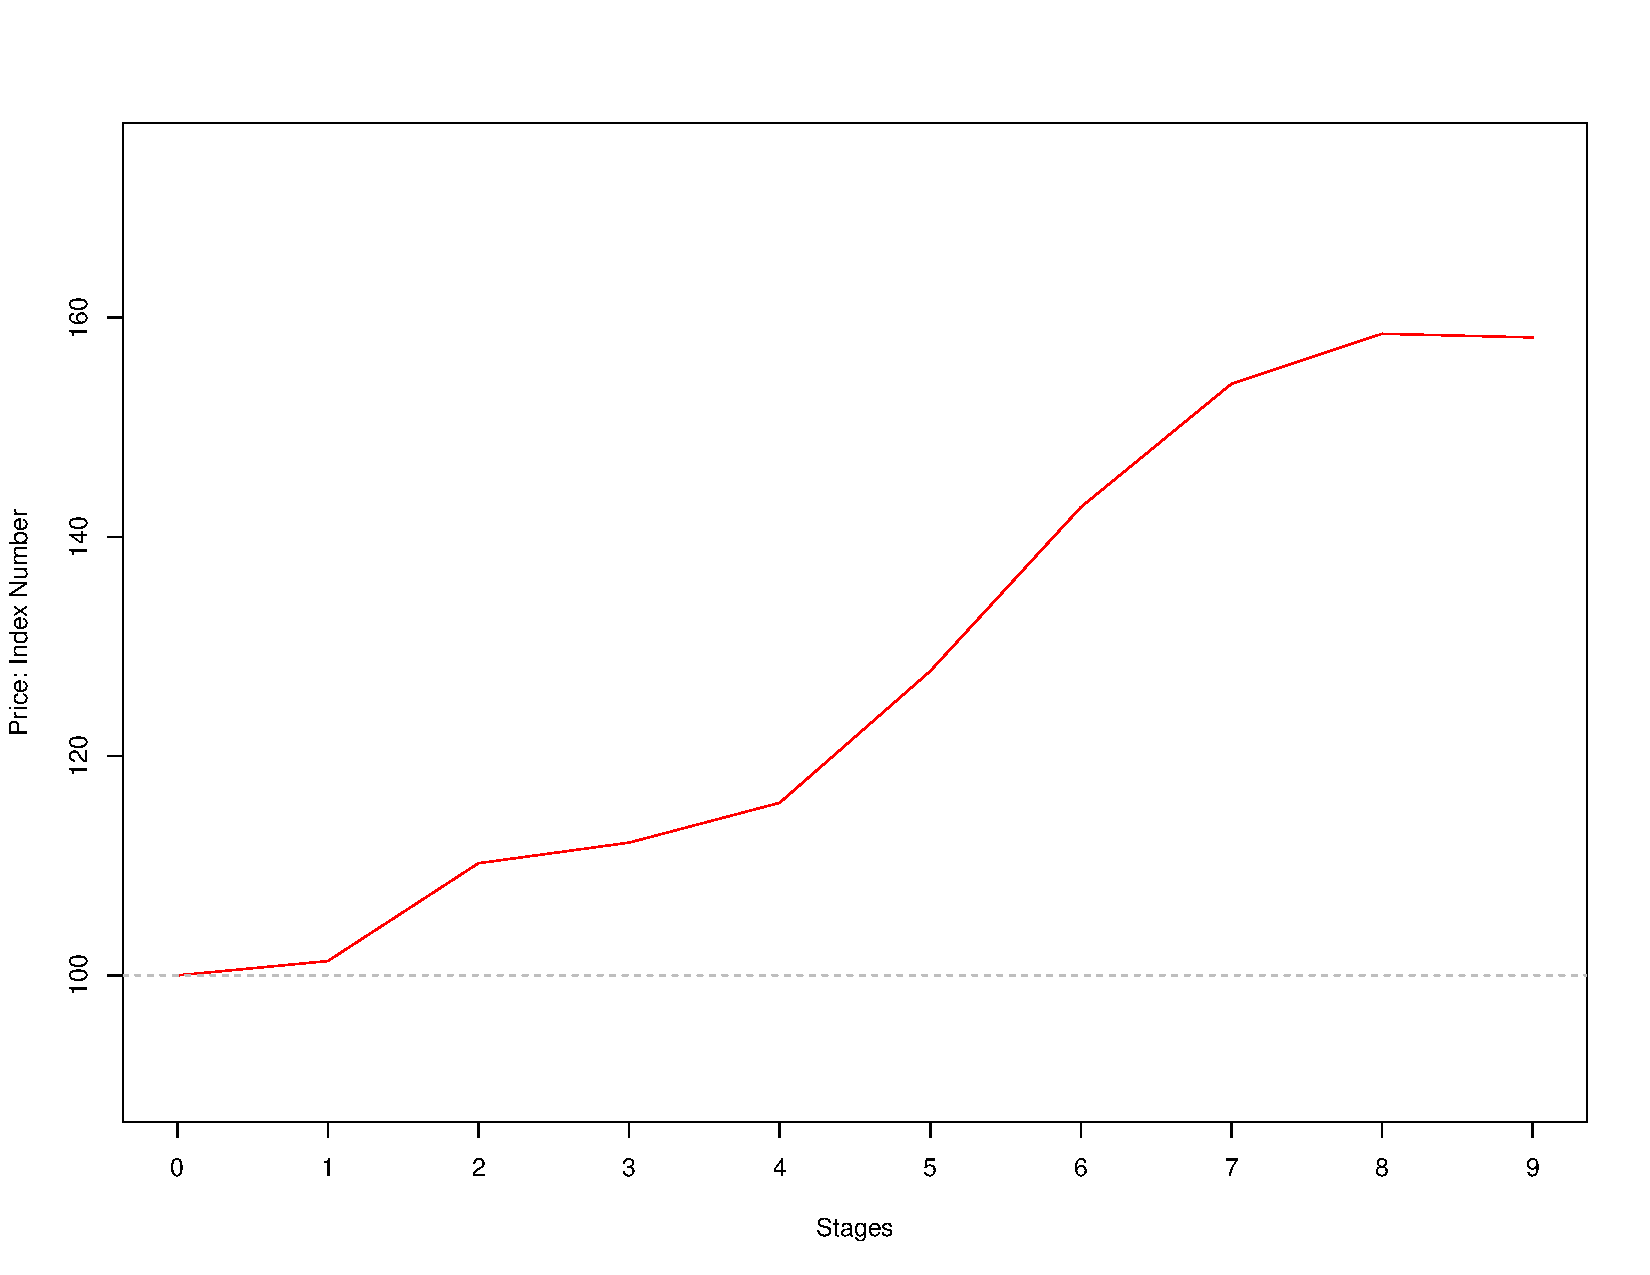
\includegraphics[scale=0.4]{laspeyres_new.pdf}
	\caption{Laspeyres index evolution for the prices of several energy resources for the period 2005-2015.}
	\label{laspeyres}
\end{figure}


\vspace*{0.15 cm}\noindent\textbf{Paasche index in R}

\noindent Analogously, the joint evolution of magnitudes under the Paasche index (\ref{niPaasche}) can be also determined by using \pkg{IndexNumber} package in R software. More specifically, \verb|paasche.index.number()| provides the mentioned weighted index number. The results of the function follows a similar structure as the function previously mentioned, and using the same graphical and numerical options. 

\begin{example}
paasche.index.number(ECResources[,2:6],ECResources[,7:11],
                     name="Price",opt.plot=TRUE,opt.summary=TRUE)
\end{example}

\vspace*{0.15 cm}\noindent\textbf{Marshall-Edgeworth index in R}

\noindent The obtaining of the Marshall-Edgeworth index number (\ref{niEdgeworth}) is also possible in R software through the use of \pkg{IndexNumber} package. In particular, we have to use the function \verb|edgeworth.index.number()| with the above-mentioned options for obtaining graphics and summaries.

\begin{example}
edgeworth.index.number(ECResources[,2:6],ECResources[,7:11],
                       name="Price",opt.plot=FALSE,opt.summary=FALSE)
\end{example}

\vspace*{0.15 cm}\noindent\textbf{Fisher index in R}

\noindent Here, we consider the case of determining the Fisher index (\ref{niFisher}). In this case, \verb|fisher.index.number()| provides a measure of the considered magnitude. Again, the options \verb|opt.plot| and \verb|opt.summary| allow the obtaining of additional information that may be of interest to the user.

\begin{example}
fisher.index.number(ECResources[,2:6],ECResources[,7:11],
                    name="Price",opt.plot=FALSE,opt.summary=FALSE)
\end{example}

\vspace*{0.15 cm}\noindent\textbf{A complex index for $v$ in R}

\noindent The complex index for $v$ given in (\ref{nivalue}) can be easily obtained as the Bradstreet-Dûtot index for the value in each instant of time. Recall that the value is obtained as the product of the amount of good by its price in each instant of time. Thus, the function \verb|aggregated.index.number()| provides the value of this new index number as follows.

\begin{example}
aggregated.index.number(ECResources[,2:6]*ECResources[,7:11],
                        base="serie",type="BDutot",name="Prices",opt.plot=FALSE,
                        opt.summary=FALSE)
\end{example}

%\section{Another section}
%
%This section may contain a figure such as Figure~\ref{figure:rlogo}.
%
%\begin{figure}[htbp]
%  \centering
%  
\includegraphics{Rlogo-5}
%  \caption{The logo of R.}
%  \label{figure:rlogo}
%\end{figure}
%
%\section{Another section}
%
%There will likely be several sections, perhaps including code snippets, such as:
%
%\begin{example}
%  x <- 1:10
%  result <- myFunction(x)
%\end{example}
%
%\section{Summary}
%
%This file is only a basic article template. For full details of \emph{The R Journal} style and information on how to prepare your article for submission, see the \href{https://journal.r-project.org/share/author-guide.pdf}{Instructions for Authors}.


\section{Concluding Remarks}
This paper discusses the implementation in R of classical index numbers used for comparing magnitudes mainly in economic contexts. Therefore, the \pkg{IndexNumber} package provides R users a set of functions to calculate   index numbers. Concretely, this library allows the calculation of simple index numbers in series and in chain. Furthermore, complex index numbers are also implemented. In particular, the non-weigthed index numbers included are the Sauerbeck, Geometric mean, Harmonic mean, Bradstreet-Dûtot, Carli, Jevons, and Dûtot indexes; as weighted index numbers, the Laspeyres, Paasche, Marshall-Edgeworth, Fisher, and Bradstreet-Dûtot indexes were considered. Additionally, this package contains graphical tools in order to facilitate the results visualization and four real data sets that can be used as illustrative examples. Moreover, the use of this library could be easily combined with other classical packages focused on time series analysis.  Future research and development plans for forthcoming versions of the package include the addition of new index numbers already considered in the  literature that can be dealt with in the framework presented above. Of course, the corresponding graphical tools should also be  implemented.




\section{Acknowledgments}
	A. Saavedra-Nieves acknowledges the financial support of FEDER/Ministerio de Ciencia, Innovaci\'on y Universidades - Agencia Estatal de Investigaci\'on under grant MTM2017-87197-C3-3-P. P. Saavedra-Nieves acknowledges the financial support of Ministerio de Eco\-nom{\'i}a y Competitividad of the Spanish government under grants MTM2016-76969-P and MTM2017-089422-P, and by the Xunta de Galicia through the European Regional Development Fund (Grupos de Referencia Competitiva ED431C-2017/38).\\



\bibliography{saavedra}



\address{Alejandro Saavedra-Nieves\\
Departamento de Estatística, Análise Matemática e Optimización\\
Universidade de Santiago de Compostela\\
  Spain\\
  ORCID: 0000-0003-1251-6525\\
  \email{alejandro.saavedra.nieves@usc.es}}

\address{Paula Saavedra-Nieves\\
	Departamento de Estatística, Análise Matemática e Optimización\\
	Universidade de Santiago de Compostela\\
	Spain\\
	  ORCID: 0000-0002-3224-8858\\
	\email{paula.saavedra@usc.es}}
